% % % % % % % % % % % % % % % % % % % % % % % % % % % % % % % % % % % % % % % % % % % %
%                                                                                     %
% Short Sectioned Assignment LaTeX Template Version 1.0 (5/5/12)                      %
% This template has been downloaded from: http://www.LaTeXTemplates.com               %
%                                                                                     %
% Original author:  Frits Wenneker (http://www.howtotex.com)                          %
%                                                                                     %
% Modified by: Fco Javier Sueza Rodríguez (fcosueza@disroot.org)                      %
%                                                                                     %
% Changes:                                                                            %
%	    - Custom Chapters, Sections and Subsections (titlesec package)                %
%           - Document type scrbook (oneside)                                         %
%           - Use babel-lang-spanish package and marvosym                             %
%           - Use hyperref, enumitem, tcolorbox and glossaries packages               %
%           - Use Time New Roman (mathptmx), Helvetic and Courier fonts               %
%                                                                                     %
% License: CC BY-NC-SA 3.0 (http://creativecommons.org/licenses/by-nc-sa/3.0/)        %
%                                                                                     %
% % % % % % % % % % % % % % % % % % % % % % % % % % % % % % % % % % % % % % % % % % % %

%-----------------------------------------------%
%	              Packages                  %
%-----------------------------------------------%

\documentclass[paper=a4, fontsize=11pt, oneside]{scrbook}

% ---- Text Input/Output ----- %

\usepackage[T1]{fontenc}
\usepackage[utf8]{inputenc}
\usepackage{mathptmx}
\usepackage[scaled=.92]{helvet}
\usepackage{courier}
\usepackage[indent=12pt]{parskip}

\usepackage{geometry}
\geometry{verbose,tmargin=3cm,bmargin=3cm,lmargin=2.6cm,rmargin=2.6cm}

% ---- Language ----- %

\usepackage[spanish]{babel}
\usepackage{marvosym}

% ---- Another packages ---- %

\usepackage{amsmath,amsfonts,amsthm}
\usepackage{graphics,graphicx}
\usepackage{titlesec}
\usepackage{fancyhdr}
\usepackage{tcolorbox}
\usepackage{hyperref}
\usepackage{enumitem}
\usepackage[automake]{glossaries}

%--------------------------------------------------------------------%
%                      Customizing Document                          %
%--------------------------------------------------------------------%


% ----------- Custom Chapters, Sections and Subsections -------------- %

\titleformat{\chapter}[display]
			{\bfseries\Huge}
			{Tema \ \thechapter} {0.5ex}
			{\vspace{1ex}\centering}

\titleformat{\section}[hang]
			{\bfseries\Large}
			{\thesection}{0.5em}{}

\titleformat{\subsection}[hang]
			{\bfseries\large}
			{\thesubsection}{0.5em}{}

\titleformat{\subsubsection}[hang]
			{\bfseries\large}
			{\thesubsubsection}{0.5em}{}

\hypersetup{
    colorlinks=true,
    linkcolor=black,
    urlcolor=magenta
}

% ------------------- Custom heaaders and footers ------------------- %

\pagestyle{fancyplain}

\fancyhead[]{}
\fancyfoot[L]{}
\fancyfoot[C]{}
\fancyfoot[R]{\thepage}

\renewcommand{\headrulewidth}{0pt} % Remove header underlines
\renewcommand{\footrulewidth}{0pt} % Remove footer underlines

\setlength{\headheight}{13.6pt} % Customize the height of the header

% --------- Numbering equations, figures and tables ----------------- %

\numberwithin{equation}{section} % Number equations within sections
\numberwithin{figure}{section} % Number figures within sections
\numberwithin{table}{section} % Number tables within sections

% ------------------------ New Commands ----------------------------- %

\newcommand{\horrule}[1]{\rule{\linewidth}{#1}} % Create horizontal rule command


%----------------------------------------------------------------------------------------
%	TÍTULO Y DATOS DEL ALUMNO
%----------------------------------------------------------------------------------------

\title{
\normalfont \normalsize
\textsc{{\bfseries Curso 2022-2023} \\ Ciclo Superior de Desarrollo de Aplicaciones Web \\ IES Aguadulce} \\ [25pt]
\horrule{0.5pt} \\[0.4cm]
\huge Formación y Orientación Laboral \\
\horrule{0.5pt} \\[0.4cm]
}

\author{Francisco Javier Sueza Rodríguez}
\date{\normalsize\today}

%----------------------------------------------------------------------------------------
%                                     DOCUMENTO
%----------------------------------------------------------------------------------------

\makeglossaries
\loadglsentries{glossary.tex}

\begin{document}

\maketitle

\newpage

\tableofcontents

\listoffigures

%\listoftables

\newpage

\chapter{Búsqueda de Empleo}
En este tema vamos a ver en que consiste la búsqueda de empleo y que herramientas y técnicas tenemos a nuestra disposición para hacer que este proceso tenga mas probabilidades de éxito. En este aspecto hay que poner de relieve la importancia de la \textbf{auto-orientación}, definida como:

<<El proceso por el cuál una persona se dota de los instrumentos y la formación necesaria para elaborar alternativas profesionales, evaluando y eligiendo aquella que se considere mejor para nuestra carrera profesional>>\cite{apuntes01}

Además, estudiaremos las salidas laborales de las titulaciones de DAW, DAM y ASIR, el perfil y la carrera profesional de estos ciclos formativos y la importancia de la formación continua dentro del desarrollo profesional.

\section{Los Ciclos Formativos de DAW, DAM y ASIR}
Los Ciclos Formativos de \textbf{DAW} (Desarrollo de Aplicaciones Web), \textbf{DAM} (Desarrollo de Aplicaciones Multiplataforma) y \textbf{ASIR} (Administración de Sistemas Informáticos en Red), pertenecientes de la familia de Informática y Telecomunicaciones, son Ciclos Formativos de Grado Superior, enmarcados dentro de la enseñanza superior.

Estos títulos capacitan para el desempeño de una profesión tanto por cuenta propia como por cuenta ajena, en el sector público o en el privado, en el ámbito TIC para el que esta pensado cada título. Cada uno de estos ciclos esta especializado en un área concreta, a saber:

 \begin{itemize}
 	\item \textbf{DAM}: centrado en el área de desarrollo de aplicaciones multiplataforma en diferentes ámbitos, como gestión empresarial, ocio, dispositivos móviles,..etc
 	\item \textbf{DAW}: que capacita para desempeñar un trabajo en el área de desarrollo en entornos Web (intranet, internet y/o extranet)
 	\item \textbf{ASIR}: este ciclo se centra en la gestión y administración de datos y la infraestructura de red de las empresas.
 \end{itemize}

\subsection{El Título}
 Los Ciclos Formativos de Grado Superior están enmarcados dentro de la Educación Superior del sistema educativo español y por lo tanto regulados por la \textbf{Ley Orgánica de Educación}, promulgada en 2006 y modificada en 2020.

 Más concretamente, el título de \textbf{ASIR} fue aprobado por el \textbf{Real Decreto 1629/2009}, publicado en el BOE el miércoles 18 de noviembre de 2009. El título de \textbf{DAM} fue aprobado en el \textbf{Real Decreto 450/2010} y publicado en el BOE el jueves 20 de mayo. Por último, el título de \textbf{DAW} fue aprobado por el \textbf{Real Decreto 686/2010} y publicado en el BOE el sábado 12 de junio de 2010.



 Los elementos básicos que identifican a estos títulos son los siguientes:

 \begin{enumerate}
    \item \textbf{Denominación}: \textbf{Desarrollo de Aplicaciones Multiplataforma}, \textbf{Desarrollo de Aplicaciones Web} y \textbf{Administración de Sistemas Informáticos en Red}
    \item \textbf{Nivel}: Formación Profesional de Grado Superior
    \item \textbf{Duración}: 2000 horas
    \item \textbf{Familia Profesional}: Informática y Telecomunicaciones
    \item \textbf{Referente Europeo}: CINE-5b (Clasificación Internacional Normalizada de Educación)
\end{enumerate}

 Estos títulos tiene validez en todo el territorio nacional, independientemente de las diferencias en su desarrollo entre las diferentes comunidades autónomas.

 Los ciclos formativos están compuestos de asignaturas, que en la formación profesional de denominan \textbf{módulos profesionales}. Los diferentes módulos que conforman los títulos de DAM, ASIR y DAM son los siguientes:

\begin{center}
 \begin{table}[ht]
    {\renewcommand{\arraystretch}{1.5}
        \begin{tabular}[c]{ |l|l| }
            \hline
            \multicolumn{2}{|c|}{\textbf{Desarrollo de Aplicaciones Web}} \\ \hline
            Sistemas Informáticos & Desarrollo Web en Entorno Servidor \\ \hline
            Bases de Datos & Despliegue de Aplicaciones Web \\ \hline
            Programación & Empresa e Iniciativa Emprendedora \\ \hline
            Lenguajes de Marcas y Sistemas de Gestión de la Información & Proyecto de Desarrollo Web\\ \hline
            Entornos de Desarrollo & Formación y Orientación Laboral \\ \hline
            Desarrollo en el Entorno Cliente & Formación en Centros de trabajo \\ \hline
            Desarrollo de Interfaces WEB &  \\ \hline
    \end{tabular}}
 \end{table}

 \begin{table}[ht]
    {\renewcommand{\arraystretch}{1.5}
        \begin{tabular}[c]{ |l|l| }
            \hline
            \multicolumn{2}{|c|}{\textbf{Desarrollo de Aplicaciones Multiplataforma}} \\ \hline
            Sistemas Informáticos &  Entornos de Desarrollo\\ \hline
            Bases de Datos & Desarrollo de Interfaces \\ \hline
            Programación & Sistemas de Gestión Empresarial \\ \hline
            Lenguajes de Marcas y Sistemas de Gestión de la Información & Proyecto de Desarrollo Multiplataforma \\ \hline
            Programación de Servicios y Procesos & Empresa e Iniciativa Emprendedora \\ \hline
            Acceso a Datos & Formación y Orientación Laboral \\ \hline
            Programación Multimedia y Dispositivos Móviles & Formación en Centro de Trabajo \\ \hline
    \end{tabular}}
 \end{table}


 \begin{table}[ht]
    {\renewcommand{\arraystretch}{1.5}
        \begin{tabular}[c]{ |l|l| }
            \hline
            \multicolumn{2}{|c|}{\textbf{Administración de Sistemas Informáticos en Red}} \\ \hline
            Implantación de Sistemas Operativos &  Implantación de Aplicaciones Web\\ \hline
            Administración de Sistemas Gestores de Bases de Datos & Planificación y administración de Redes \\ \hline
            Fundamentos de Hardware & Seguridad y Alta Disponibilidad \\ \hline
            Lenguajes de Marcas y Sistemas de Gestión de la Información & Formación y Orientación Laboral \\ \hline
            Gestión de Bases de Datos & Proyecto de Administración de Sistemas \\ \hline
            Acceso a Datos & Empresa e Iniciativa emprendedora \\ \hline
            Servicios de Red e Internet & Formación en Centro de Trabajo \\ \hline
    \end{tabular}}
 \end{table}
\end{center}

Para información sobre la normativa que regula los títulos de de Formación Profesional y en concreto los visto en esta sección podemos consultar las siguientes enlaces:

\begin{itemize}
    \item \href{https://www.boe.es/buscar/doc.php?id=BOE-A-2006-7899}{Ley Orgánica de Educación}
    \item \href{https://www.boe.es/boe/dias/2010/05/20/pdfs/BOE-A-2010-8067.pdf}{Real Decreto 450/2010} - \textbf{DAW}
    \item \href{https://www.boe.es/boe/dias/2010/06/12/pdfs/BOE-A-2010-9269.pdf}{Real Decreto 686/2010} - \textbf{DAM}
    \item \href{https://www.boe.es/boe/dias/2009/11/18/pdfs/BOE-A-2009-18355.pdf}{Real Decreto 1629/2009} - \textbf{ASIR}
\end{itemize}

\subsection{El futuro de tus estudios}
En la sociedad actual, cada vez es mas necesario para las empresas el acceso y la organización de la información. Para llevar esto a cabo, se necesitan aplicaciones que permitan gestionar dicha información de manera íntegra. Así mismo, el uso cada vez mas extendido de dispositivos electrónicos como PDAs, móviles, tablets y el acceso a internet de la mayoría de la población demanda la creación de aplicaciones especificas.

El perfil de \textbf{desarrollador de software} (multiplataforma o web) se encarga de la creación de estas aplicaciones, proporcionando una mayor integración de los sistema de gestión e intercambio de información en las diferentes plataformas así como asegurando la integridad, consistencia y accesibilidad de los datos empleados. También es trabajo del desarrollador tener en cuenta parámetros como la usabilidad, que facilitan la interacción del usuario con la aplicaciones, y la adaptación a nuevas técnicas y entornos de desarrollo específicos para la aplicaciones que se quieren desarrollar.

En el caso del \textbf{administrador de sistemas informáticos en red}, su labor consiste en una mayor integración, en la pequeña y mediana empresa, de la integración de los sistema de gestión de la información	así como la intervención en sistemas informáticos destinados a la producción y el apoyo al resto de departamentos de una organización.

Por lo tanto, todo parece indicar que el futuro de la profesión esta garantizado, ya que cada vez se necesitan mas profesionales con perfiles técnicos y específicos debido a que los requerimientos cada vez de vuelven mas complejos y se precisan personas mejor preparadas.

Si quieres ampliar la información, puedes consultar los siguientes enlaces:

\begin{itemize}
    \item \href{https://administracionelectronica.gob.es/pae_Home?_nfpb=true&_pageLabel=P1200733131296129097704&langPae=es#faq1}{Centro de Transferencia de Tecnología}
    \item \href{https://educacionadistancia.juntadeandalucia.es/formacionprofesional/mod/scorm/player.php?a=6198&scoid=178876&currentorg=eXe68448_2zip5d5bab14269131fb5c2&mode=&attempt=1}{Cursos de Especialización FP}
\end{itemize}

Por último, cabe recordar que actualmente, la \textbf{profesión esta evolucionando} con unas características concretas, dirigiéndose hacia:

\begin{itemize}
    \item Una \textbf{mayor integración} de los \textbf{sistemas de gestión} en intercambio de información basados en diferentes plataformas y tecnologías.
    \item Una \textbf{mayor demanda de asistencia técnica} a través de la \textbf{tele-operación}, asistencia técnica remota y asistencia <<on line>>.
    \item La \textbf{adaptación de los desarrolladores} a nuevas técnicas y entornos de desarrollo por el aumento en el consumo de teléfonos, PDA y dispositivos móviles.
    \item El\textbf{ apoyo a otros departamentos} dentro de la empresa asegurando la funcionalidad y rentabilidad del sistema informático.x
\end{itemize}


\subsection{Los técnicos superiores en los centros de trabajo}
Los Técnicos Superiores en DAW, DAM y ASIR desempeñan su labor tanto en la empresa pública como en la privada, aunque lo más común es que sea en el sector privado donde desarrollan su actividad.

Tanto los titulados en \textbf{DAM} como en \textbf{DAW} desempeñan su trabajo en el área de desarrollo de aplicaciones en diversos ámbitos, estando el primero mas enfocado al desarrollo en diferentes plataformas incluyendo los dispositivos móviles mientras en segundo se centra más en la plataforma web. Respecto a los titulados en \textbf{ASIR}, su labor consiste en el aseguramiento de la funcionalidad y rentabilidad del sistema informático, asistencia local y remota,..etc.

Aunque no es lo más frecuente, los Técnicos de DAM, DAW y ASIR pueden desempeñar sus funciones en las administración pública estatal, autonómica o local. Aunque no siempre es necesario tener aprobada una oposición, esta es la vía más común de acceso a estos puestos.

Según un estudio publicado por Infoempleo, los profesionales que han cursado estudios de grado superior de FP son mas demandados que los que han cursado grado medio, con un porcentaje de 57\% y 47\% respectivamente. Estos datos de inserción son muy positivos e indican que los perfiles se adecuan a los actuales requerimientos del mercado laboral.\cite{educaweb}

\subsection{El nivel académico}
Los títulos de Técnico Superior (DAW, DAM y ASIR) forman parte del Sistema Educativo Español promulgado por la Ley Orgánica de Educación y se enmarcan dentro de las Enseñanzas Superiores y de la Formación Profesional de Grado Superior. Por lo tanto, se trata de unos \textbf{estudios superiores}, solo por detrás de los estudios universitarios.

Para acceder a un Grado Superior es necesario cumplir alguna de los siguientes requisitos:
\begin{enumerate}[label={\alph*.}]
    \item Estar en posesión del título de Bachiller
    \item Poseer el título de Técnico de grado medio y haber superado un curso de formación específico para el acceso a ciclos de grado superior en centros públicos o privados autorizados por la administración educativa
    \item Haber superado una prueba de acceso. En este supuesto, se requerirá tener diecinueve años, cumplidos en el año de realización de la prueba o dieciocho si se acredita estar en posesión de un título de Técnico relacionado con aquél al que se desea acceder
    \item Haber superado la Prueba de Acceso de la Universidad para mayores de 25, se requerirá tener cumplidos 25 años en el momento de realización de la prueba.
\end{enumerate}

Para más información sobre los requisitos de acceso, cupos y equivalencias, se puede consultar la pagina de la \href{https://www.juntadeandalucia.es/educacion/portals/web/formacion-profesional-andaluza/quiero-formarme/ensenanzas/fp-grado-superior/requisitos}{Consejería de Educación} de la Junta de Andalucía.

Es conveniente reseñar que dado el nivel superior de estudios, el nivel \textbf{\gls{actitudinal}}, \textbf{\gls{procedimental}} y \textbf{\gls{conceptual}} requerido corresponderá con ello, y todo el proceso de enseñanza de ve influenciado por esta característica.

Cabe también destacar que el nivel académico superior posibilita un \textbf{sistema de convalidaciones} de módulos del Ciclo Formativo con asignaturas o materias de de enseñanza universitarias, basado en un sistema de créditos ECTS y en los acuerdos entre las Consejerías de Educación y las Universidades.

En el apartado 3 de la Disposición adicional primera, <<Colaboración entre la formación profesional superior y la enseñanza universitaria>>, la \href{https://www.boe.es/boe/dias/2011/03/12/pdfs/BOE-A-2011-4551.pdf}{Ley Orgánica 4/2011}, de 11 de marzo, complementaria de la Ley de Economía Sostenible, podrás consultar la normativa más actual en relación a las convalidaciones de módulos y materias universitarias.

\subsection{El nivel profesional}
Los Ciclos Formativos de Formación profesional tienen como objetivo desarrollar las competencias generales correspondientes a la \textbf{\gls{cualificacion}} o cualificaciones objetos de estudio en dicho título.

Desde un punto de vista profesional, la cualificación es un conjunto de \textbf{\gls{competencias}} profesionales (conocimientos y capacidades) que dan respuesta a ocupaciones y puestos de trabajo con valor en el mercado laboral, y que pueden adquirirse mediante la formación o la experiencia laboral. Las cualificaciones profesionales son el referente de los títulos de Formación Profesional.

El conjunto de cualificaciones profesionales vienen recogidas en el Catálogo Nacional de Cualificaciones Profesionales (\textbf{CNCP}) que determina el Instituto Nacional de Cualificaciones (\textbf{INCUAL}) a través de un proceso de análisis productivo.

Las cualificaciones se clasifican en 5 niveles profesionales en función de la complejidad y destreza en los conocimientos y capacidades en las competencias que se alcanzan. En concreto, los \textbf{Técnicos Superiores} se enmarcan dentro del\textbf{ nivel 3} de esta clasificación que se define de la siguientes forma:

<<Competencia en un conjunto de actividades profesionales que requieren el dominio de diversas técnicas y puede ser ejecutado de forma autónoma. Comporta responsabilidad de coordinación y supervisión de trabajo técnico y especializado. Exige la comprensión de los fundamentos técnicos y científicos de las actividades y la evaluación de los factores del proceso y de sus repercusiones económicas.>>

Toda esta teoría se aplica tanto al sector público como al privado.

En el \textbf{sector público} se establece una clasificación de los funcionarios en base a la Ley 7/2007, de 12 de abril, del Estatuto Básico del Empleado Público, donde se reconocen los siguientes grupos:

\begin{itemize}
    \item \textbf{Grupo A}: Graduados Universitarios
    \item \textbf{Grupo B}: Técnicos Superiores de la FP
    \item \textbf{Grupo C1}: Técnicos de FP y Bachilleres
    \item \textbf{Grupo C2}; Titulados en ESO
\end{itemize}

Tanto en el {\bfseries sector privado} como sí el trabajador de la administración pública no es personal funcionario, la clasificación se rige por los \textbf{\gls{convenios colectivos}}, que se tratarán con mas profundidad en otros temas.

\section{Salidas Profesionales}
El sector de la informática y las nuevas tecnologías esta en constante evolución. Los trabajadores en este sector suelen tener una gran vocación y creatividad, que les permite dar soluciones satisfactorias a los diferentes problemas que se les van planteando. Además, el contacto con el cliente es cada vez mas directo lo que hace que tengan que ser buenos comunicadores con gran capacidad de dialogo y negociación.

Como futuro profesional del sector debes conocer la peculiaridades del entorno laboral en que tendrás que desenvolverte, por eso en este apartado analizaremos las características del empleo en el sector de la informática y especialmente las salidas laborales que existen.

\subsection{Características Generales del Sector de la Informática}
Todos los sectores tienen unas características propias que los definen, el sector de la informática y las nuevas tecnologías no es menos. A continuación se listan las principales características de este sector:

\begin{itemize}
    \item La informática y las nuevas tecnologías son una realidad en nuestras vidas, por ello la \textbf{demanda de profesionales} que puedan ayudarnos en su uso y mantenimiento es una \textbf{constante} tanto en el ámbito empresarial como en el particular.
    \item Es un sector donde los cambios y la innovación son constantes, por ello se necesitan \textbf{profesionales} que estén en \textbf{continuo reciclaje} y sean capaces del \textbf{autoaprendizaje}. La formación continua es clave en el sector.
    \item La \textbf{empresa privada} es la principal \textbf{fuente de empleo} para el sector. Aunque la administración pública es consumidora del mismo, no suele convocar oposiciones para cubrir estos puestos, sino que contrata empresas externas.
    \item Es un \textbf{sector} que esta en \textbf{auge} ya que la mayoría de las empresa usan, en mayor o menor medida, nuevas tecnologías.
\end{itemize}

\subsection{Salidas Profesionales en el Sector Privado}
En el sector de la informática y las nuevas tecnologías la empresa privada es al que ofrece más posibilidades de colocación. A continuación mostramos una lista con los puestos mas relevantes que pueden ocupar los diferentes técnicos:

\begin{itemize}
    \item \textbf{Técnico Superior en de Aplicaciones Multiplataforma}:
    \begin{itemize}
        \item Desarrollador de aplicaciones informáticas para la gestión empresarial y de negocio.
        \item Desarrollador de aplicaciones de propósito general.
        \item Desarrollador de aplicaciones en el ámbito del entretenimiento y la informática móvil.
    \end{itemize}
    \item \textbf{Técnico Superior en Desarrollo de Aplicaciones Web}:
    \begin{itemize}
        \item Desarrollador de aplicaciones Web.
        \item Programador Web.
        \item Programador Multimedia.
    \end{itemize}
    \item \textbf{Técnico Superior en Administración de Aplicaciones en Red}:
    \begin{itemize}
        \item Técnico en administración de sistema.
        \item Responsable de informática.
        \item Técnico de servicio de internet.
        \item Técnico de servicios de mensajería electrónica.
        \item Personal de apoyo y soporte técnico.
        \item Técnico de teleasistencia.
        \item Técnico de administración de bases de datos.
        \item Técnico de redes.
        \item Supervisor de Sistemas.
        \item Técnico de servicios de comunicaciones.
        \item Técnico de entornos web.
    \end{itemize}
 \end{itemize}

Para todos estos puestos se buscan trabajadores que tengan capacidad de trabajo en equipo ya que la mayoría de proyectos se desarrollan en equipos que debe estar perfectamente coordinado. También se buscan personas flexibles y creativas, adaptables a los cambios tecnológicos y con facilidad de aprender nuevos lenguajes de programación.

\subsection{Salidas Profesionales en el Sector Público}
El cuerpo de \textbf{Técnicos Auxiliares de Informática} de la Administración del Estado se crea con carácter de cuerpo general interministerial en 1990 adscribiéndose al Ministerio de Administraciones Públicas. Este cuerpo esta clasificado dentro del \textbf{Grupo C1}, por lo que para acceder a estas plazas se necesita tener un título de Bachiller o equivalente. Los perfiles idóneos son los Técnicos Superiores en Desarrollo Multiplataforma, Desarrollo de Aplicaciones Web y Administradores de Sistemas en RED.

Las funciones desempeñadas por los miembros del \textbf{Cuerpo de Técnicos Auxiliares de Informática} son un parte esencial en el desarrollo y mantenimiento de los sistemas informáticos automatizados de la Administración General el Estado. Entre sus funciones se encuentra el análisis y programación de aplicaciones, apoyo a los usuarios,  mantenimiento de hardware, instalación de equipos y sistemas, operación de sistemas de grandes bases de datos,.. entre otros.

Es una opción interesante que también se puede contemplar, aunque hay muchas más posibilidades de encontrar empleo en el sector privado.

\subsection{El Autoempleo}
Una alternativa al trabajo por cuenta ajena es el \textbf{autoempleo}, montar tu propia empresa, organizarte como emprendedor/a.

Antes de continuar con el desarrollo de esta sección cabe destacar que en el currículo de estos módulos profesionales se incluye el módulo \textbf{Empresa e Iniciativa Emprendedora}, destinado específicamente al desarrollo de las ideas del autoempleo, por lo que que vamos a ver en esta sección se verá ampliado y desarrollado en este módulo.

Las posibilidades de organizar una empresa en el ámbito de la informática y las TIC presenta una serie de oportunidades que podemos resumir en las siguientes:

\begin{itemize}
    \item El \textbf{capital inicial} que se precisa es, en términos relativos, bajo.
    \item En uso de las tecnologías por parte de las empresas y particulares hace que haya una \textbf{demanda importante de técnicos} que puedan resolver de forma rápida y eficiente los problemas que van surgiendo con el uso de estas tecnologías.
    \item Existe la posibilidad de acceder a \textbf{financiación pública} a través de subvenciones y ayudas de las distintas administraciones.
\end{itemize}

Las oportunidades son importantes, no obstante hay que saber valorar que no basta con que existan buenas oportunidades para que un proyecto empresarial o de autoempleo alcance el éxito. Es necesario\textbf{ poseer la cualidades} y capacidades técnicas que requiere el trabajo autónomo, tales como iniciativa, capacidad de liderazgo, resistencia a la presión, conocimientos generales de gestión de empresas, mucha capacidad de trabajo, autoorganización y autocontrol.

Respecto al apartado económico, el capital inicial va a ser necesario, aunque en este sector se tratan de cantidades que una persona de nivel económico medio, o incluso bajo, pueda llegar a alcanzar, ya que la \textbf{inversión inicial} necesaria es \textbf{baja} en comparación con otro tipo de negocios. Además, se puede recurrir a la \textbf{financiación ajena}, por medio de un banco, por ejemplo, y optar a \textbf{subvenciones al autoempleo} que puede ser una buena ayuda, especialmente al principio.

\section{El Perfil Profesional de los Técnicos de DAM, DAW y ASIR}
En cada puesto de trabajo se piden una capacidades, conocimientos, destrezas y actitudes necesarias para llevar al cabo la actividad que se va a desarrollar. En este punto vamos a analizar estos aspectos relativos a la titulación que estamos estudiando, basándonos en el Real Decreto que aprueba el título. Para la elaboración de los títulos se han llevado a cabo completo análisis del mercado laboral evaluando las competencias requeridas por las empresas del Sector de la Informática y las TIC.

En el Real Decreto se establece el \textbf{\gls{perfil profesional}} de los títulos de DAW, DAM y ASIR, determinando su \textbf{competencia general}, así como sus \textbf{competencias profesionales}, \textbf{personales} y \textbf{sociales}, puntos que discutiremos en las siguientes secciones con mas detalle.

Para completar esta información, sería conveniente hablar con profesionales que trabajen en el sector para que nos hablen de su experiencia, que se pide de ellos, que les cuesta mas trabajo, etc...

\subsection{La Competencia General}
El perfil profesional de DAW, DAM y ASIR queda determinado, como hemos comentado, por sus competencias, pero también por la relación de cualificaciones y, en su caso, por la unidades de competencia del \textbf{Catálogo Nacional de Cualificaciones}, el cuál es un compendio de las profesiones que están vigentes en el actual sistema productivo español y que está elaborado por el \textbf{Instituto Nacional de Cualificaciones} (INCUAL).

La \textbf{competencia general} de DAM consiste en desarrollar, implantar, documentar y mantener aplicaciones multiplataforma, utilizando tecnologías y entornos de desarrollo específicos, garantizando la accesibilidad de los datos de forma segura y cumpliendo los estándares de usabilidad y calidad exigidos.

La \textbf{competencia general} DAW consiste en desarrollar, implantar, documentar y mantener aplicaciones web, con independencia del modelo empleando y usando tecnologías específicas, asegurando el acceso a los datos de forma segura y cumpliendo con los criterios de accesibilidad, usabilidad y calidad exigidos en los estándares.

La \textbf{competencia general} ASIR consiste en configurar, administrar y mantener sistemas informáticos, garantizando la funcionalidad, la integridad de los recursos y servicios del sistema, con la calidad exigida y cumpliendo con la legislación vigente.

Estas competencias generales se desarrollan en varias cualificaciones profesionales que comprenden una serie de unidades de competencia del Catálogo Nacional de Cualificaciones Profesionales.

El técnico en \textbf{Desarrollo de Aplicaciones Multiplataforma}, según el Catalogo Nacional de Cualificaciones, podrá configurar y explotar sistemas informáticos, programar bases de datos relacionales, desarrollar componentes software en lenguajes de programación estructurada y orientados a objetos. También podrá instalar y configurar sistema de planificación de recursos empresariales.

El técnico en \textbf{Desarrollo de Aplicaciones Web} podrá desarrollar elementos de software en el entorno cliente, en el entorno servidor e implementar, verificar y documentar aplicaciones en internet, intranet y extranet. También podrá configurar y explotar sistemas de planificación de recursos empresariales.

El técnico en \textbf{Administración de Sistemas Informáticos en Red} podrá administrar los dispositivos hardware del sistema, podrá instalar, configurar y administrar bases de datos, aplicaciones de sistema, software de entorno web, servicios de mensajería electrónica, servicios de transferencia de archivos y multimedia. También podrá asegura los equipos informáticos y configurar y explotar los sistemas informáticos en general, así como implementar, documentar y verificar aplicaciones web en entornos internet, intranet y extranet.

\subsection{Competencias Profesionales}
Una vez vistas la competencias general, vamos a ver la competencias profesionales que establece el Real Decreto que define cada título:

\begin{itemize}
    \item \textbf{Desarrollo de Aplicaciones Multiplataforma}:
    \begin{itemize}
        \item \textbf{Configurar y explotar sistemas informáticos}, adaptando la configuración lógica según las necesidades de uso y los criterios establecidos.
        \item \textbf{Aplicar técnicas y procedimientos} relacionados con la \textbf{seguridad} en sistemas, servicios y aplicaciones y cumpliendo el plan de seguridad.
        \item \textbf{Gestionar bases de datos}, interpretando su diseño lógico y verificando integridad, consistencia, seguridad y accesibilidad de los datos.
        \item \textbf{Gestionar entornos de desarrollo} adaptando su configuración en cada caso para permitir el desarrollo y despliegue de aplicaciones.
        \item \textbf{Desarrollar aplicaciones multiplataforma} con acceso a bases de datos utilizando lenguajes, librerías y herramientas adecuados.
        \item \textbf{Integrar contenidos gráficos} y \textbf{componentes multimedia} en aplicaciones multiplataforma, empleando herramientas específicas y cumpliendo los requerimientos específicos.
        \item \textbf{Desarrollar interfaces gráficos de usuario interactivos }y con la usabilidad adecuada, empleando componentes visuales estándar o implementando componentes visuales específicos.
        \item Participar en el \textbf{desarrollo de juegos y aplicaciones} en el \textbf{ámbito de entretenimiento} y la educación empleando técnicas, motores y entornos de desarrollo específicos.
        \item \textbf{Desarrollar aplicaciones} para \textbf{teléfonos},\textbf{ PDA} y \textbf{otros dispositivos móviles} empleando técnicas y entornos de desarrollo específicos.
        \item \textbf{Crear ayudas generales} y sensibles al contexto, empleando herramientas específicas e integrándolas en sus correspondientes aplicaciones.
        \item\textbf{ Crear tutoriales},\textbf{ manuales de usuario}, \textbf{de instalación},\textbf{ de configuración} y \textbf{de administración}, empleando herramientas específicas.
        \item \textbf{Empaquetar aplicaciones para su distribución} preparando paquetes auto instalables con asistentes incorporados.
        \item \textbf{Desarrollar aplicaciones multiproceso y multihilo} empleando librerías y técnicas de programación específicas.
        \item \textbf{Desarrollar aplicaciones} capaces de ofrecer \textbf{servicios en red} empleando mecanismos de comunicación.
        \item Participar en la \textbf{implantación de sistemas ERP-CRM} evaluando la utilidad de cada uno de sus módulos.
        \item \textbf{Gestionar la información} almacenada en \textbf{sistemas ERP-CRM} garantizando su integridad.
        \item \textbf{Desarrollar componentes} personalizados para un \textbf{sistema ERP-CRM} atendiendo a los requerimientos.
        \item \textbf{Realizar planes de pruebas} verificando el funcionamiento de los componentes de software desarrollados, según especificaciones.
        \item \textbf{Desplegar y distribuir aplicaciones} en distintos ámbitos de implantación verificando su comportamiento y realizando las modificaciones necesarias.
    \end{itemize}
    \item \textbf{Desarrollo de Aplicaciones Web}:
    \begin{itemize}
        \item \textbf{Configurar y explotar sistemas informáticos}, adaptando la configuración lógica del sistema según las necesidades de uso y los criterios establecidos.
        \item \textbf{Aplicar técnicas y procedimientos} relacionados con la \textbf{seguridad} en sistemas, servicios y aplicaciones, cumpliendo el plan de seguridad.
        \item \textbf{Gestionar servidores de aplicaciones} adaptando su configuración en cada caso para permitir el despliegue de aplicaciones web.
        \item \textbf{Gestionar bases de datos}, interpretando su diseño lógico y verificando integridad, consistencia, seguridad y accesibilidad de los datos.
        \item \textbf{Desarrollar aplicaciones web} con acceso a bases de datos utilizando lenguajes, objetos de acceso y herramientas de mapeo adecuados a las especificaciones.
        \item \textbf{Integrar contenidos} en la lógica de una \textbf{aplicación web}, desarrollando componentes de acceso a datos adecuados a las especificaciones.
        \item \textbf{Desarrollar interfaces en aplicaciones web} de acuerdo con un \textbf{manual de estilo}, utilizando lenguajes de marcas y estándares web.
        \item \textbf{Desarrollar componentes multimedia} para su \textbf{integración en aplicaciones web}, empleando herramientas específicas y siguiendo las especificaciones establecidas.
        \item \textbf{Integrar componentes multimedia} en el interface de una aplicación web, realizando el análisis de interactividad, accesibilidad y usabilidad de la aplicación.
        \item \textbf{Desarrollar e integrar componentes software} en el \textbf{entorno del servidor web}, empleando herramientas y lenguajes específicos, para cumplir las especificaciones de la aplicación.
        \item \textbf{Desarrollar servicios} para integrar sus funciones en otras aplicaciones web, asegurando su funcionalidad.
        \item \textbf{Integrar servicio}s y \textbf{contenidos distribuidos} en aplicaciones web, asegurando su funcionalidad.
        \item \textbf{Completar planes de pruebas} verificando el funcionamiento de los componentes software desarrollados, según las especificaciones.
        \item \textbf{Elaborar y mantener la documentación} de los procesos de desarrollo, utilizando herramientas de generación de documentación y control de versiones.
        \item \textbf{Desplegar y distribuir aplicaciones web} en distintos ámbitos de implantación, verificando su comportamiento y realizando modificaciones.
        \item\textbf{ Gestionar y/o realizar el mantenimiento} de los recursos de su área en función de las cargas de trabajo y el plan de mantenimiento.
    \end{itemize}
    \item \textbf{Administración de Sistemas en Red}:
    \begin{itemize}
        \item \textbf{Administrar sistemas operativos de servidor}, instalando y configurando el software, en condiciones de calidad para asegurar el funcionamiento del sistema.
        \item \textbf{Administrar servicios de red} (web, mensajería electrónica y transferencia de archivos, entre otros) instalando y configurando el software, en condiciones de calidad.
        \item \textbf{Administrar aplicaciones} instalando y configurando el software, en condiciones de calidad para responder a las necesidades de la organización.
        \item\textbf{ Implantar y gestionar bases de datos} instalando y administrando el software de gestión en condiciones de calidad, según las características de la explotación.
        \item \textbf{Optimizar el rendimiento del sistema} configurando los dispositivos hardware de acuerdo a los requisitos de funcionamiento.
        \item \textbf{Evaluar el rendimiento} de los \textbf{dispositivos hardware} identificando posibilidades de mejoras según las necesidades de funcionamiento.
        \item \textbf{Determinar} la \textbf{infraestructura de redes} telemáticas elaborando esquemas y seleccionando equipos y elementos.
        \item \textbf{Integrar equipos de comunicaciones} en infraestructuras de redes telemáticas, determinando la configuración para asegurar su conectividad.
        \item \textbf{Implementar soluciones de alta disponibilidad}, analizando las distintas opciones del mercado, para proteger y recuperar el sistema ante situaciones imprevistas.
        \item \textbf{Supervisar la seguridad física} según especificaciones del fabricante y el plan de seguridad para evitar interrupciones en la prestación de servicios del sistema.
        \item \textbf{Asegurar el sistema y los datos} según las necesidades de uso y las condiciones de seguridad establecidas para prevenir fallos y ataques externos.
        \item \textbf{Administrar usuarios} de acuerdo a las especificaciones de explotación para garantizar los accesos y la disponibilidad de los recursos del sistema.
        \item \textbf{Diagnosticar las disfunciones} del sistema y \textbf{adoptar las medidas} correctivas para restablecer su funcionalidad.
        \item \textbf{Gestionar y/o realizar el mantenimiento de los recursos} de su área (programando y verificando su cumplimiento), en función de las cargas de trabajo y el plan de mantenimiento.
    \end{itemize}
\end{itemize}

\subsection{Competencias Personales y Sociales}
Ya hemos visto las competencias generales y las profesionales, en este último punto veremos las \textbf{personales y sociales}. En este sentido, aspectos como la \textbf{autoconfianza}, las \textbf{habilidades sociales}, la \textbf{participación}, la \textbf{autonomía} y la \textbf{iniciativa} son actitudes que tiene un valor primordial en cualquier puesto de trabajo.

El R.D del Título de Técnico Superior en \textbf{Desarrollo de Aplicaciones Multiplataforma} establece las siguientes competencias personales y sociales \cite{rd686}:

\begin{itemize}
    \item \textbf{Establecer vías eficaces} de \textbf{relación profesional} y \textbf{comunicación} con sus superiores, compañeros y subordinados, respetando la autonomía y competencias de las distintas personas.
    \item \textbf{Liderar  situaciones  colectivas}  que  se  puedan  producir, \textbf{mediando} en conflictos personales  y  laborales,  \textbf{contribuyendo}  al  establecimiento  de  un  \textbf{ambiente  de  trabajo agradable}, actuando en todo momento de forma respetuosa y tolerante.
    \item \textbf{Gestionar su carrera profesional}, analizando las oportunidades de empleo, autoempleo y de aprendizaje.
    \item Mantener el \textbf{espíritu de innovación y actualización} en el ámbito de su trabajo para adaptarse a los cambios tecnológicos y organizativos de su entorno profesional.
    \item \textbf{Crear y gestionar una pequeña empresa}, realizando un \textbf{estudio de viabilidad} de productos, de \textbf{planificación} de la producción y de comercialización.
    \item \textbf{Participar de forma activa} en la vida económica, social y cultural, con una actitud crítica y responsable
\end{itemize}

El R.D del Título de Técnico Superior en \textbf{Desarrollo de Aplicaciones Web} establece las siguientes competencias personales y sociales \cite{rd450}:

\begin{itemize}
    \item\textbf{ Resolver situaciones}, problemas o contingencias con \textbf{iniciativa y autonomía} en el ámbito de su competencia, con creatividad, innovación y espíritu de mejora en el trabajo personal y en el de los miembros del equipo.
    \item \textbf{Organizar y coordinar equipos de trabajo}, supervisando el desarrollo del mismo, con responsabilidad, manteniendo relaciones fluidas y asumiendo el liderazgo, así como, aportando soluciones a los conflictos grupales que se presentan.
    \item \textbf{Comunicarse con sus iguales}, superiores, clientes y personas bajo su responsabilidad\textbf{ utilizando vías eficaces de comunicación}, transmitiendo la información o conocimientos adecuados, y respetando la autonomía y competencia de las personas que intervienen en el ámbito de su trabajo.
    \item \textbf{Generar entornos seguros} en el \textbf{desarrollo de su trabajo} y \textbf{el de su equipo}, supervisando y aplicando los procedimientos de prevención de riesgos laborales y ambientales de acuerdo con lo establecido por la normativa y los objetivos de la empresa.
    \item \textbf{Supervisar y aplicar procedimientos}  de  \textbf{gestión  de  calidad}, de \textbf{accesibilidad universal} y de \textbf{diseño para todos}, en las actividades profesionales incluidas en los procesos de producción o prestación de servicios.
    \item \textbf{Realizar la gestión básica} para la \textbf{creación y funcionamiento de una pequeña empresa}  y  tener  iniciativa en su actividad profesional con sentido de la responsabilidad social.
    \item \textbf{Ejercer sus derechos} y \textbf{cumplir con las obligaciones} derivadas de su actividad profesional, de acuerdo con lo establecido en la legislación vigente, participando activamente en la vida económica, social y cultural.
\end{itemize}

El R.D del Título de Técnico Superior en \textbf{Administración de Sistemas Informáticos en Red} establece las siguientes competencias personales y sociales \cite{rd1629}:

\begin{itemize}
    \item \textbf{Efectuar consultas}, dirigiéndose \textbf{a la persona adecuada} y saber respetar la autonomía de los subordinados, informando cuando sea conveniente.
    \item \textbf{Mantener el espíritu de innovación y actualización} en el ámbito de su trabajo para adaptarse a los cambios tecnológicos y organizativos de su entorno profesional.
    \item \textbf{Liderar  situaciones colectivas} que se puedan producir, \textbf{mediando en conflictos} personales y laborales, contribuyendo al establecimiento de un ambiente de trabajo agradable y actuando en todo momento de forma sincera, respetuosa y tolerante.
    \item \textbf{Resolver problemas} y tomar \textbf{decisiones individuales}, siguiendo las normas y procedimientos establecidos, definidos dentro del ámbito de su competencia.
    \item \textbf{Gestionar su carrera profesional}, analizando las oportunidades de empleo, autoempleo y de aprendizaje.
    \item \textbf{Participar de forma activa} en la vida económica, social y cultural con actitud crítica y responsable.
    \item \textbf{Crear y gestionar una pequeña empresa}, realizando un estudio de viabilidad de productos, de planificación de la producción y de comercialización
\end{itemize}

Hay que tener en cuenta que las competencias personales y sociales se han añadido recientemente a los currículos de los diferentes estudios, ya que antes solo se tenía en cuenta los aspectos conceptuales y el aprendizaje memorístico.

En la siguiente lista, se resumen las los \textbf{requerimientos actitudinales} necesarios para tu trabajo:

\begin{itemize}
        \item \textbf{Ser una persona}:
        \begin{itemize}
            \item Capaz de comunicar con claridad.
            \item Capaz de negociar.
            \item Empática.
            \item Respetuosa.
            \item Asertiva.
            \item Tolerante.
            \item Dialogante.
            \item Que practique la escucha activa.
            \item Con iniciativa.
            \item Creativa.
            \item Eficaz y eficiente.
        \end{itemize}
        \item \textbf{Saber}:
        \begin{itemize}
            \item Realizar y recibir críticas constructivas.
            \item Gestionar las emociones.
            \item Compartir.
        \end{itemize}
\end{itemize}

Ya hemos visto todas las competencias que se necesitan para desarrollar la actividad en un puesto de trabajo en del Sector de la Informática, en la siguientes sección, hablaremos de la carrera profesional, como hacer un balance de nuestra carrera, tomar decisiones o definir nuestros objetivos profesionales.

\section{La Carrera Profesional}
La carrera profesional se trata de \textbf{los diferentes puestos de trabajo} que vamos ocupando a lo largo de nuestra \textbf{vida profesional} y que van \textbf{evolucionando} con el tiempo.

<<El concepto de carrera profesional a la secuencia evolutiva de experiencias de trabajo de una persona a lo largo del tiempo>> (Arthur, Hall y Lawrence, 1989).

En la actualidad ha quedado atrás la idea de que una persona pase toda su vida trabajando en el mismo puesto de trabajo, actualmente, ya sea por motivos económicos, psicológicos o por los cambios en el sistema de producción, los trabajadores suelen cambiar de empresa, de tipo de empleo y se recualifican, es decir, evolucionan.

Por este motivo, es importante que planifiquemos nuestro futuro profesional para tomar las decisiones acertadas y llegar al punto en que queremos estar. Este proceso puede empezar con la realización de 4 preguntas simples:

\begin{itemize}
    \item ¿Que soy, profesionalmente hablando?
    \item ¿Que hay en el mercado de trabajo?
    \item ¿Que busco en el mundo laboral?
    \item ¿Cómo busco lo que quiero alcanzar?
\end{itemize}

\subsection{Balance Personal}
Para responder a la primera pregunta tenemos que hacer una análisis de nuestra capacidades profesionales, lo que llamamos un \textbf{Balance Personal}. Para llevarlo a cabo podemos usar diferentes herramientas, aunque nosotros nos vamos a centrar en un instrumento sencillo y eficaz que es el currículum, pero uno especial que vamos a llamar \textbf{Currículum en Bruto}.

Para realizar este \textbf{currículum en bruto}, vamos a seguir los siguientes pasos:

\begin{enumerate}
    \item Partiendo de una plantilla sencilla de currículum, vamos a añadir algún apartado. Los aspectos que incluyen son:
    \begin{itemize}
        \item \textbf{Datos Personales}: nombre y apellidos, teléfono, dirección, etc...
        \item \textbf{Datos Académicos}: todos los estudios realizados desde el colegio hasta el último titulo que tengamos, incluyendo fechas de realización, duración y centro donde lo cursamos.
        \item \textbf{Formación Complementaria}: aquí pondremos todo tipo de cursos que hayamos realizado, especificando fechas, duración, centros..
        \item \textbf{Idiomas}: especificación del nivel de idiomas tanto hablado como escrito.
        \item \textbf{Experiencia Profesional}: detallaremos todos los trabajos que hemos tenido, su duración, empresas, tipo de contrato, funciones...
        \item \textbf{Experiencia con contenido profesional}: detallaremos actividades que hayamos realizado que puedan tener valor como contenido profesional, como realización de deportes, ayuda en negocio familiar, actividades de voluntariado,...
        \item \textbf{Informática}: nivel de manejo informático.
        \item \textbf{Actitudes y Aptitudes Positivas}: aspectos como la capacidad de sacrificio, ganas de trabajar o capacidad de aprendizaje. Aquí se pueden usar tests de orientación profesional.
        \item \textbf{Aspectos a mejorar}: debemos incluir aquellas aptitudes y actitudes que no las tenemos suficientemente desarrolladas. Igualmente que en el punto anterior, podemos usar test de orientación laboral.
    \end{itemize}

    Para analizar nuestros aspectos negativos y positivos podemos realizar una lista o una tabla con dos secciones, Aspectos Positivos y Negativos, y rellenarla.

    \item Una vez elaborada la lista de aspectos positivos y negativos, pregúntate si el resto de la gente te ve así. Es posible que tengamos una percepción equivocada, por lo que podrías preguntar a 3 o 4 compañeros o gente con la que suelas trabajar que escriban una lista con los aspectos positivos que ven en tí.

    \item Por último, se tiene que recordar que al hacer un currículum extenso tiene un valor de autoconocimiento, por lo que ademas de hacer una labor de recuerdo y recopilación de nuestro historial profesional, debemos ser especialmente sinceros.
\end{enumerate}

Para ayudarte en la realización de algunos puntos de este currículum, o simplemente si quieres mejorar tu autoconocimiento, puedes visitar la web \href{https://www.psicoactiva.com/test/diagnosticos/}{Psicoactiva.com} donde encontrarás una gran variedad de test en los que apoyarte.

\subsection{El Análisis el Mercado de Trabajo}
Una vez que hemos analizado nuestras capacidades profesionales, es momento de que analicemos el mercado laboral para ver que oportunidades ofrece. Para realizar un análisis del mercado laboral podemos seguir los siguientes pasos:

\begin{enumerate}
    \item \textbf{Consultar fuentes ya elaboradas}, como algunas de las siguientes:
    \begin{itemize}
        \item \textbf{Encuesta de Población Activa (EPA)}: encuesta de carácter trimestral y que es el mayor y mas riguroso análisis del Mercado de Trabajo que se realiza en nuestro país. En la página web del INE podemos consultar la \href{https://www.ine.es/dyngs/INEbase/es/operacion.htm?c=Estadistica_C&cid=1254736176918&menu=ultiDatos&idp=1254735976595}{última EPA}, perteneciente al segundo trimestre de 2022.
        \item \textbf{Estudios de Mercado laboral de ámbito municipal}: muchos ayuntamientos publican resultados de encuestas de la situación laboral del municipio. Tienen la ventaja de que nos ofrecen una visión de nuestro entorno más cercano.
        \item \textbf{Estudios sectoriales de mercado}: son estudios que analizan la situación de un sector concreto del Mercado Laboral,
    \end{itemize}
    \item \textbf{Consultar fuentes de información directa}, siendo las mas frecuentes:
    \begin{itemize}
        \item Las ofertas de empleo que salen en \textbf{Webs de empleo}.
        \item Las \textbf{ofertas de empleo público} que publican ayuntamientos, comunidades autónomas y el estado central.
        \item Las ofertas de empleo que salen publicadas en la prensa, especialmente en la prensa local.
        \item Nuestra \textbf{red de contactos}, a la que podemos movilizar preguntando activamente sobre las posibilidades laborales en nuestra área de interés.
    \end{itemize}
    \item Una vez \textbf{recopilados todos los datos obtenidos}, los \textbf{valoramos} y \textbf{extraemos las conclusiones} sobre el mercado laboral que nos interesen o influyan directamente.
\end{enumerate}

Para encontrar mas información estadística sobre el tema, podemos consultar la \href{https://www.ine.es/}{Página Web del INE}, que es la mayor fuente estadística de España.

\subsection{Definición de un Objetivo Profesional}
Una vez que hemos valorados nuestras capacidades y realizado un análisis del mercado laboral es el momento de definir nuestros objetivos profesionales. Definir un objetivo consiste en \textbf{definir las ocupaciones} o \textbf{puestos de trabajo} en función de \textbf{nuestras capacidades}, \textbf{intereses} y el \textbf{mercado laboral}.

El objetivo profesional debe cumplir las siguientes características:

\begin{itemize}
    \item Debe ser \textbf{realista y alcanzable}, si nos proponemos objetivos demasiado ambiciosos corremos el riesgo de desmotivarnos.
    \item Tiene que tener cierto grado de \textbf{flexibilidad}, de manera que no nos cierre oportunidades, pero que tenga una concreción suficiente para que nos sirva de guía.
    \item Ha de apoyarse en una \textbf{secuencia temporal}, que suele se uno, tres y cinco años. No conviene fijarse objetivos superiores a los 5 años.
    \item Ha de incluir un \textbf{plan de acción concreto}, el cual veremos en el siguiente apartado.
\end{itemize}

Definir los objetivos es complicado, pero una vez tomada la decisión, si se es constante para alcanzar la meta es una de las claves para el éxito profesional.

\subsection{El Plan de Acción}
La siguiente fase consiste en la elaboración de un plan de acción, el cuál estará condicionado a la decisión que ya has tomado de estudiar un Ciclo Formativo de Grado Superior, y ha de ser coherente con esta elección. Independientemente de esto se pueden hacer más cosas o enfocar tus estudios de diferentes formas.

El \textbf{plan de acción} pude apoyarse en los siguientes aspectos:

\begin{itemize}
    \item Identificar los \textbf{ámbitos de mejora}: necesidad de formación especializada, necesidad de mejora de las capacidades personales, necesidad de ganar experiencia laboral, mejora en idiomas, etc...
    \item Definir \textbf{actividades a realizar}: en función de los ámbitos de mejora que hayas definido habrá que buscar actividades que ayuden a mejorarlos, como buscar cursos, mejorar el manejo de ciertas herramientas informáticas, etc...
    \item Realizar una \textbf{temporalización}: se trata de fijar fechas de comienzo y finalización de las actividades que te has propuesto.
\end{itemize}

El plan de empleo debe ser concreto, pero a la vez flexible. Un error común es plantearse demasiadas actividades a las que no se pueden atender convenientemente y se dejan a la mitad. Para evitar estas situaciones hay que hacer un \textbf{ejercicios de realismo} con nuestras posibilidades y ajustarse a ellas.

\section{¿Que Hacer tras Finalizar el Ciclo?}
La Formación Profesional prepara a los alumnos/as para la actividad en el campo profesional y facilita su adaptación  las modificaciones laborales que se puedan producir a lo largo de su vida profesional, así como a contribuir a su desarrollo personal y al aprendizaje permanente.

En este punto veremos cuales son las posibilidades tras acabar el ciclo formativo que estas cursando. Ademas de para trabajar, el ciclo te abre un abanico de posibilidades formativas, como se puede ver en la siguiente figura.

\begin{figure}[ht]
    \centering
    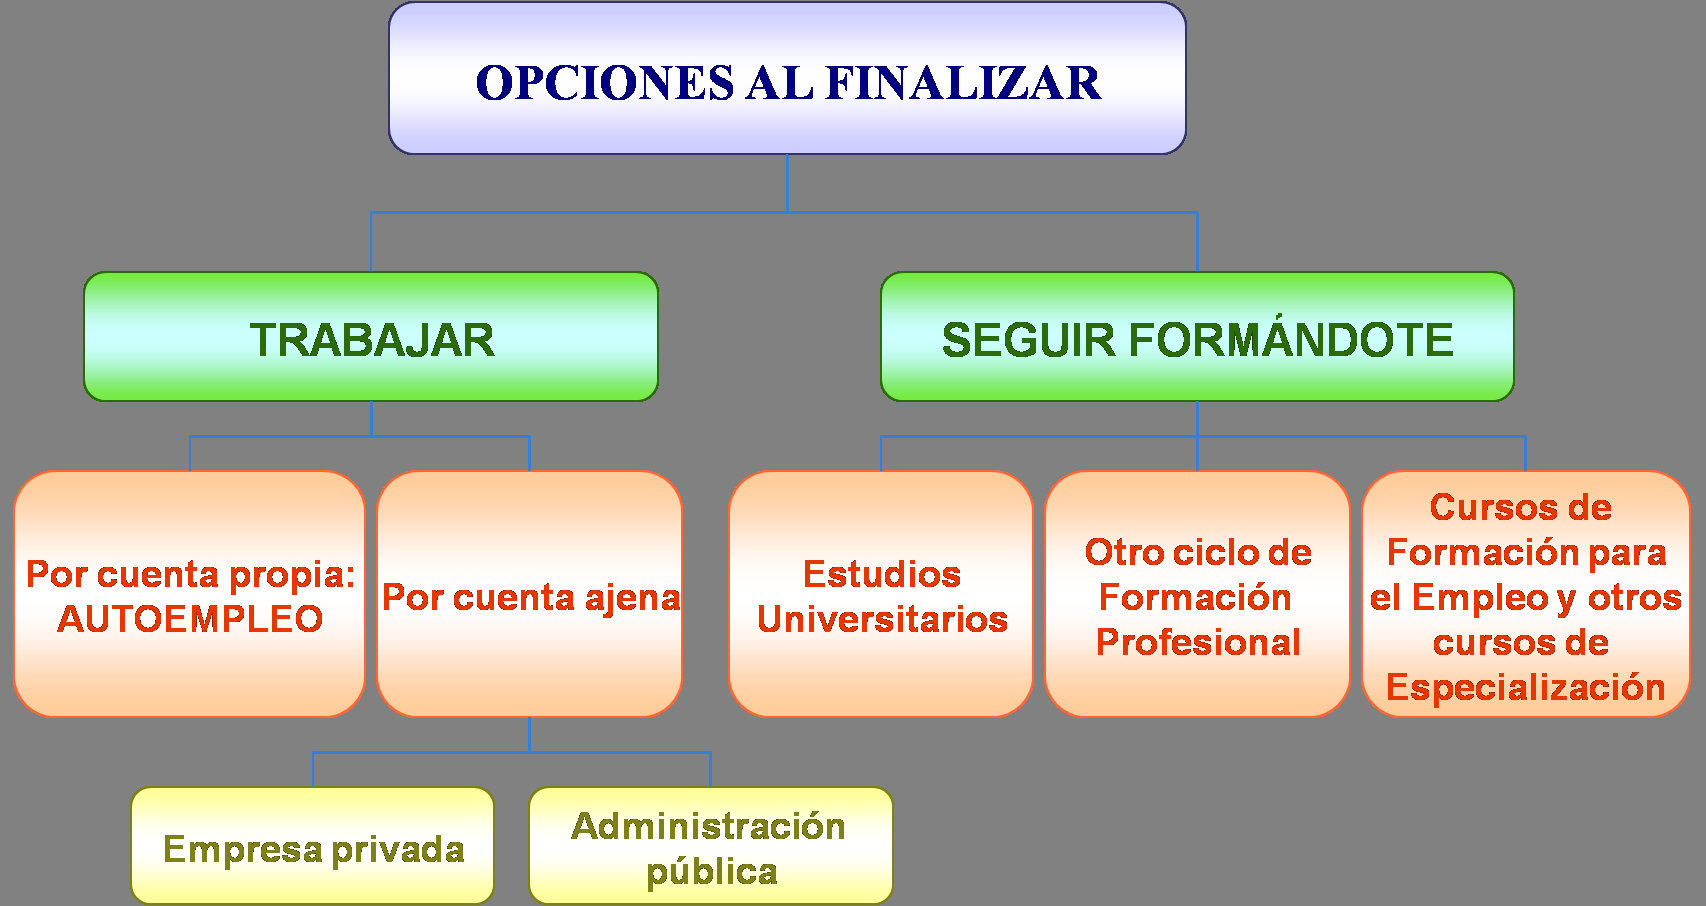
\includegraphics[scale=0.30]{esquema-FP.png}
    \caption{Salidas después de acabar un Ciclo Superior}
\end{figure}

Como vemos en el esquema hay muchas posibilidades tras acabar tus estudios. Puedes seguir formándote, ya sea haciendo otro módulo, accediendo a la universidad o realizando cursos de formación para el empleo. También puede lanzarte al mercado laboral, ya sea por cuenta propia o por cuenta ajena. Dependiendo de las opción que tomes, deberás informarte de sus requerimientos, algunos de los cuales no se logran de la noche a la mañana.

Por lo tanto, lo primero es fijarte unos objetivos, para lo que es necesario que conozcas el proceso de toma de decisiones, que veremos en el siguiente punto.

\section{La Toma de Decisiones}
La \textbf{toma de decisiones} es el \textbf{proceso} por el cuál se realiza \textbf{una elección} entre \textbf{las alternativas} para resolver diferentes situaciones de la vida. Consiste, básicamente, en elegir una alternativa de entre las disponibles a los efectos de resolver un problema.

Aunque no existe una receta infalible, antes de tomar una decisión que afecta a tu futuro es conveniente que analices todas las posibilidades.

\subsection{Fases de la Toma de Decisiones}
Dentro del proceso de toma de decisiones podemos diferenciar varias fases, las cuales son las siguientes:

\begin{itemize}
    \item \textbf{Reconocimiento}: la toma de decisiones comienza cuando se presenta una nueva situación de oportunidades o amenazas. Para que se pueda considerar una toma de decisiones debe haber al menos dos alternativas entre las que escoger.
    \item \textbf{Enumeración de las alternativas/opciones}: en esta etapa se definirán cuales son las alternativas y opciones, las cuales dependerán de tus metas y tus valores. Tener consciencia de tus prioridades y valores es muy importante y te ayudará a definir tus metas y alternativas. En esta fase ayuda hacer una lista con todas las opciones y alternativas.
    \item \textbf{Análisis/Evaluación de Alternativas}: en esta fase es necesario analizar las alternativas, usando la lista elaborada en el punto anterior, teniendo en cuenta las opciones que ofrece cada alternativa, así como sus ventajas he inconvenientes. Habrá también que analizar los recursos que requiere cada alternativa así como los beneficios esperados de está.

    Algo que nos puede ayudar es elaborar un cuadro con las diferentes alternativas y sus ventajas e inconvenientes como vemos en la siguiente figura.

    \begin{figure}[ht]
        \centering
        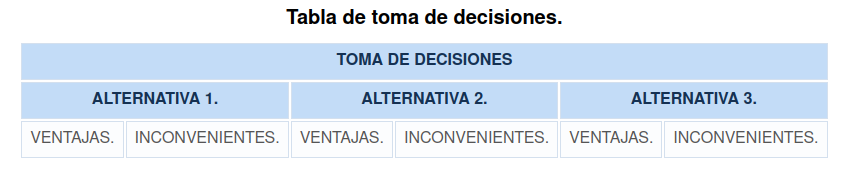
\includegraphics[scale=0.50]{tabla-decisiones.png}
        \caption{Alternativas del proceso de toma de decisiones}
    \end{figure}

    \item \textbf{Elección}: tras evaluar cada alternativa, hay que decantarse por una. Ahora deberás centrarte en ella y estudiar como ponerla en práctica, elaborando una estrategia, examinando de nuevo la información recogida sobre esta alternativa, sus posibles dificultades y como superarlas.
    \item \textbf{Ejecución}: en esta etapa se lleva a la práctica la alternativa elegida. Pueden surgir contratiempos menores, que harán vacilar, pero al final se puede llevar a cabo. En cambio, si se presentan desafíos o insatisfacciones más serías, puede abandonarse esta alternativa y volver al principio del proceso de toma de decisiones, con la ventaja de la experiencia ya ganada.
\end{itemize}

\section{¿Quieres Trabajar?}
En esta sección vamos a analizar las diferentes opciones que tenemos de empleo así como la importancia de la búsqueda activa, el currículum vitae o el proceso de selección, entre otras cosas.

\subsection{Búsqueda de Empleo: Factores de Ocupabilidad}
La búsqueda de empleo supone un gran trabajo, pero esta comprobado que las personas que se preparan una estrategia en su búsqueda de empleo aumenta su efectividad en una 70\% frente a las que no lo hacen. A la hora de elaborar una estrategia hay muchos factores que influyen en su eficacia, como la información que tengamos del mercado laboral, el nivel de formación y las posibilidades de mejorarlo, el grado de motivación y autoestima, las habilidades profesionales y personales, así como el dominio de determinadas técnicas y herramientas para la búsqueda de empleo.

Dos personas, con la misma formación y un experiencia profesional parecida pueden tener resultados muy distintos en el proceso de búsqueda de empleo. Esto se debe a que influyen una serie de factores que influyen en el proceso y que se conocen como factores de ocupabilidad.

Los \textbf{factores de ocupabilidad} son características que determinan tu forma de trabajar, de relacionarte con los demás y que las empresas consideran sumamente importantes. Parece demostrado que determinadas capacidades hacen que el rendimiento de un trabajador sea muy superior al de otro que tiene los mismos conocimientos técnicos pero que no posee estas capacidades.

Los factores de ocupabilidad se pueden clasificar en cuatro grupos \cite{trabyper}:

\begin{enumerate}
    \item \textbf{Factores estructurales}: estos factores tienen que ver con el mercado laboral al que se pretende acceder y es prácticamente imposible influir en ellos.
    \item \textbf{Factores personales}: en estos factores influyen tu experiencia y conocimiento, pero también tu edad, sexo, estado civil o algún tipo de problema físico que pueda afectar al desarrollo de tu actividad laboral.
    \item \textbf{Factores competenciales}: estos factores son los que tienen que ver con tus habilidades profesionales y es donde el entrevistador comparará tus habilidades técnicas con el resto de candidatos.
    \item \textbf{Factores psicosociales}: estos factores están influenciados por el entorno social y cultural e incluyen elementos como la disponibilidad hacia el empleo, madurez ocupacional, apoyo socio-familiar, autoimagen profesional y personal, etc...
\end{enumerate}

Por último, te proponemos realizar un cuestionario cuya finalidad es el análisis de las actitudes personales requeridas para el desempeño de un puesto de trabajo determinado. Este \href{https://www.ich.es/Empleabilidad/FactPsicoOcupa/FactPsicoOcupa.php}{cuestionario} te ayudará a conocer tus puntos débiles en este aspecto.

\subsection{El Proyecto Profesional}
El \textbf{proyecto profesional} es un documento donde identificaremos cuáles son nuestros objetivos profesionales y personales. El objetivo del mismo es evaluar tu formación, tu experiencia e identificar tus cualidades y capacidades para valorar si cumples los requisitos que el mercado laboral esta demandando en dicho momento.

Esto permite conocer de manera óptima tu personalidad y perfil profesional, orientándote en la búsqueda de empleo para seleccionar las ofertas que se ajusten a tus características.

El proyecto profesional consta de 3 fases con sus respectivos documentos, como vimos en la sección 1.4 \textit{``La Carrera Profesional''}, y que vamos a repasar en este punto. Así, las fases del proyecto profesional son las siguientes:

\begin{enumerate}
    \item \textbf{Mis aportaciones al mercado laboral (Balance Personal)}: debemos conocernos a nosotros mismos de forma que podamos vendernos a las empresas, destacando nuestra fortalezas y ``camuflando'' nuestras debilidades. Por lo que deberás hacer un listado con los aspectos positivos y negativos de tu personalidad.
    \item \textbf{Análisis del Mercado Laboral}: cuando nos decidamos por un determinado puesto de trabajo deberemos realizar una \textbf{prospección} del mercado laboral para saber cuales son los requisitos del puesto, así como que ofrecen las empresas. Una vez que hayamos recopilado la información, podemos hacer una tabla similar a la de la siguiente figura \ref{tab:emp} para ver si el puesto se ajusta a nuestro perfil profesional.

    \item \textbf{Objetivo Profesional}: una vez que conocemos lo que podemos ofrecer y lo que piden las empresas, tenemos que definir a que puestos vamos a optar, las condiciones laborales que estamos dispuestos a aceptar y elaboraremos un plan de acción para conseguir nuestro objetivo.
\end{enumerate}

\vspace{10ex}

\begin{figure}[ht]
    \centering
    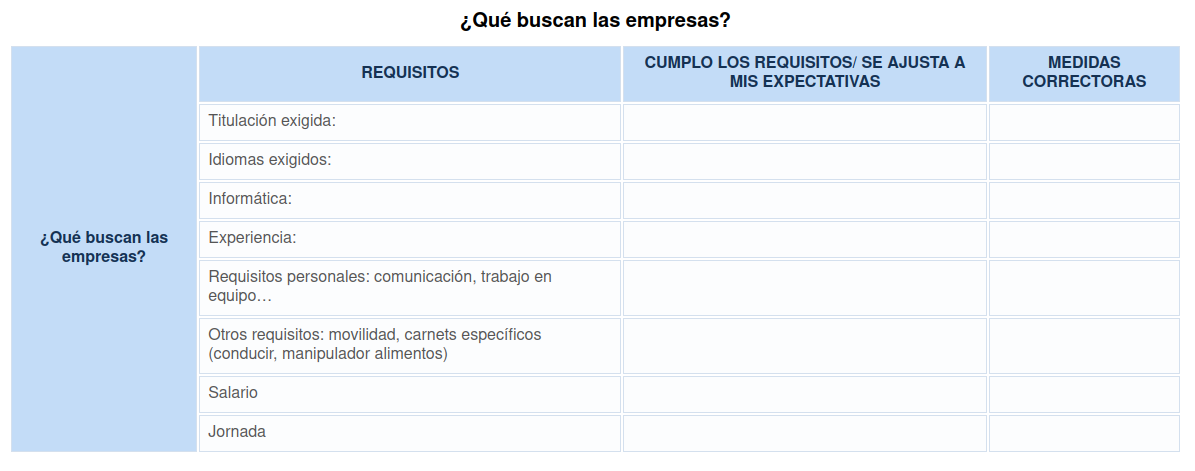
\includegraphics[scale=0.50]{tabla-empresas.png}
    \caption{Perfil profesional vs Requisitos empresas}
    \label{tab:emp}
\end{figure}

Es \textbf{importante} que consultes los siguientes modelos para ampliar la información dada en este punto y ver la estructura de un proyecto personal y un plan de empresa.

\begin{itemize}
    \item Modelo Proyecto Personal - \url{http://www.publicacions.ub.edu/liberweb/mundo_trabajo/cuestionario.pdf}
    \item Modelo Plan de Empresa - \url{https://blog.cofike.com/plan-de-empresa-ejemplo/}
\end{itemize}

También encontrar información sobre el proyecto personal con más detalle de todos los documentos implicados en cada fase en el \textbf{Anexo A.1}.

\subsection{El Proceso de Búsqueda de Empleo}
La búsqueda de empleo requiere de la utilización de un conjunto de técnicas las cuales se refieren al conocimiento, aprendizaje y mejora de todas aquellas estrategias y habilidades que enriquecen los recursos personales y aumentan la posibilidad de encontrar trabajo.

Estas técnicas no nos van a garantizar que encontremos trabajo inmediatamente pero si van a ayudar a aumentar nuestras posibilidades en la búsqueda de empleo.

La búsqueda de empleo implica llevar a cabo las siguientes acciones:

\begin{enumerate}
    \item \textbf{¿Que trabajo busco?} (Proyecto Profesional)
    \item \textbf{Localizar Ofertas} (Canales de búsqueda de empleo)
    \item \textbf{Contactar con las ofertas} (Instrumentos de presentación: carta y currículum)
    \item \textbf{Entrar en el proceso de selección} (Entrevista, Psicotécnicos,...)
    \item \textbf{Contratación} (modelos de contrato y derechos laborales)
\end{enumerate}

De la lista anterior ya hemos visto el proyecto profesional, por lo que en esta sección nos centraremos en las siguientes, salvo en los modelos de contrato y derechos laborales que se estudiarán con mas detalle en las siguientes unidades.

\subsubsection{Canales de Búsqueda de Empleo}
La búsqueda de empleo no es una tarea sencilla, y saber utilizar correctamente los diferentes canales de los que disponemos para realizarla puede facilitarnos un poco el proceso.

Podemos diferenciar dos tipos de \textbf{canales de búsqueda de empleo}, los pasivos y los activos.


\subsubsection*{Canales Pasivos}
Son canales en los que la búsqueda se deja en manos de terceros y se está a la espera de que te ofrezcan un puesto de trabajo. En este caso, entregarás un currículum o rellenarás una solicitud de empleo y se pondrán en contacto contigo cuando reciban ofertas que de adapten a tu perfil. Los principales medios de tipo de canales son:

\begin{itemize}
    \item \textbf{Agencias de Colocación Personal}: empresa destinada a poner en contacto a empresas que ofertan empleos con personas que los demanda. Puedes encontrar un directorio con una lista de consultorías y agencias de colocación en los siguientes enlaces:
    \begin{itemize}
        \item \href{https://www.infojobs.net/#seccion3}{Consultorías de Selección de Personal}
        \item \href{https://www.informacion-empresas.com/745_SELECCION-COLOCACION-PERSONAL.html}{Directorio de empresas de colocación y selección}
    \end{itemize}
    \item \textbf{Empresas de Trabajo Temporal} (ETTs): empresa que se encarga de poner a disposición de otra empresa, con carácter temporal, trabajadores que ha contratado. En el siguiente enlace puedes ver una lista del Ministerio de Trabajo con las principales ETTs.
    \begin{itemize}
        \item \href{https://expinterweb.mites.gob.es/sigett/consultaPublicaETT}{Lista de Empresas de Trabajo Temporal}
    \end{itemize}
    \item \textbf{Asociación de Técnicos de Informática}: esta asociación puede ser una vía para informarte sobre el empleo en tu campo profesional, así como acceder a su bolsa de trabajo, cursos, etc...
    \begin{itemize}
        \item \href{https://www.ati.es/}{Asociación de Técnicos de Informática}
    \end{itemize}
    \item \textbf{Bolsa de trabajo del centro en el que estudias}: muchos de los IES donde se imparten enseñanzas de formación profesional cuentan con bolsas de trabajo relacionadas con los Ciclos Formativos que imparten.
    \item \textbf{Sindicatos}, \textbf{Ayuntamientos} y otras \textbf{entidades públicas} con servicios de orientación al empleo.
    \item \textbf{Servicio Público Estatal de Empleo} (SEPE) o \textbf{servicios de colocación} de tu \textbf{Comunidad Autónoma}.
    \item \textbf{Internet}: hay un montón de páginas web dedicadas a la búsqueda de empleo, que te permiten crearte un currículum o formulario para mandarte ofertas que se adapten a tu perfil. Algunas de las más conocidas son las siguientes:
    \begin{itemize}
        \item \href{https://www.infojobs.net/}{Infojobs}
        \item \href{https://www.trabajos.com/}{Trabajos.com}
        \item \href{https://www.infoempleo.com/}{Infoempleo}
        \item \href{https://www.primerempleo.com/}{PrimerEmpleo}
        \item \href{https://www.oficinaempleo.com/}{OficinaEmpleo}
        \item \href{https://www.opcionempleo.com/}{OpciónEmpleo}
    \end{itemize}
\end{itemize}

Además de estos podemos encontrar multitud de plataformas especializadas en sectores concretos o en modos de trabajo concreto, como búsqueda de empleo para trabajar en remoto, para freelancers, trabajar en el extranjero, etc...

\subsubsection*{Canales Activos}
A diferencia de los canales pasivos, donde se requiere poca activad, en los canales activos se exige que haya más participación, debiendo intervenir en la búsqueda y selección de las ofertas de empleo, envío de currículum vitae, comunicación con familiares y amigos, etc... Los principales canales activos, son los siguientes:

\begin{itemize}
    \item \textbf{Red de Contactos Personal}: se considera que el 60\% de las ofertas de empleo no llegan a publicarse, ya que las empresas primero buscan entre sus conocidos. Esto pone de relieve la importancia de crearse una red de contactos que puedan ayudarte a encontrar empleo.
    \item \textbf{Autocandidatura o mailing}: es una variedad del marketing directo que consiste en enviar tu currículum a empresas que puedan necesitar trabajadores con tu perfil profesional. Para ello deberes buscar los datos de la empresa y enviarle tu currículo y carta de presentación a la persona responsable de las contrataciones. Suele hacerse por email.
    \item \textbf{Webs especializadas en empleo}: además de las comentadas en los canales pasivos, hay algunas webs en las que es recomendable visitarlas todos los días y consultar las ofertas que van apareciendo.
    \item \textbf{SEPE: Punto de Encuentro de Empleo}: en la web del servicio público de empleo podrás consultar las ofertas de trabajo que hay en tu provincia. En este \href{https://www.empleate.gob.es/empleo/#/trabajo?search=*&pag=0}{enlace} puedes acceder directamente al Punto de Encuentro del SEPE.
    \item \textbf{Televisión}: existen programas de televisión destinados al empleo, donde diariamente se exponen ofertas de trabajo. Uno de ellos es el programa de la 2 de TVE, \textit{``Aquí hay trabajo''}.
    \item \textbf{Prensa, radio, teletexto}: en estos medios de comunicación podrás encontrar ofertas de trabajo a las que podrás remitir tu currículum. Los domingos, especialmente, se publican suplementos sobre empleo en muchos periódicos de tirada nacional y local.
    \item \textbf{Empleo para Discapacitados}: por último, ONCE a través de su fundación FSC Inserta ofrece servicios de inserción laboral para discapacitados. No dudes en visitar su \href{https://www.insertaempleo.es/}{su página web} si tienes alguna discapacidad.
\end{itemize}

\subsubsection{Instrumentos de Presentación: Carta y Currículum}
Ahora ya tenemos claro cual es nuestro perfil laboral, hemos creado un proyecto profesional con nuestras metas y seleccionado los puestos a los que queremos optar. Además conocemos los diferentes canales donde podemos buscar empleo.

El siguiente paso es conocer dos instrumentos que nos vendrán muy bien a la hora de promocionarnos y ``vendernos'' a las empresas: \textbf{la carta de presentación} y \textbf{el currículum vitae}. Estos documentos nos precederán en cualquier empresa en la que queramos trabajar y nos servirán para diferenciarnos de nuestro competidores, aunque su principal función es \textbf{conseguirnos una entrevista} de trabajo. Por ello, deben estar redactados ajustados a las exigencias del puesto de trabajo al que quieres optar y que muestre una imagen de ti atractiva para el empleador.

\subsubsection*{La Carta de Presentación}
La \textbf{carta de presentación} se envía a aquellas empresas o lugares que pueden ofrecer oportunidades de empleo, es la ``tarjeta de visita'' que acompaña a tu currículum vitae. Su objetivo es atraer la atención de la persona que la lea, pensar que tienes un perfil perfecto para cubrir el puesto que se ofrece y animar a la lectura de tu currículum.

Las cartas de presentación de clasifican en dos tipos:

\begin{itemize}
    \item \textbf{Carta de Respuesta a una Oferta de Empleo}: esta se envía como respuesta a alguna oferta de empleo en algún medio e irá acompañando a tu currículum. Debe aludir necesariamente al anuncio en cuestión, señalando su referencia. En ella debes destacar por qué es interesante tu candidatura.
    \item \textbf{Carta de Autocandidatura}: carta que se envía por iniciativa propia a una empresa que pueda necesitar profesionales con nuestro perfil, ya sea en ese momento o en un futuro cercano. Debe explicar que te ha motivado a acercarte a la empresa y que puedes aportar. Si es interesante las empresas pueden archivarla y tenerla en cuenta en próximos procesos de selección.
\end{itemize}

Hay que tener un par de aspectos en cuenta antes de lanzarte a redactar la carta de presentación:

\begin{itemize}
    \item \textbf{Infórmate} sobre la \textbf{empresa} a la que te diriges y el \textbf{puesto} al que quieres optar. Identifica la cultura corporativa y resume los elementos claves del perfil.
    \item Intenta \textbf{averiguar} quien \textbf{realiza la selección de personal} y cual es su nombre. Así podrás dirigir la carta a esa persona concreta aumentando la probabilidad de ser leída.
\end{itemize}

En los siguientes enlaces puedes consultar diferentes modelos de carta de carta de presentación así como un resumen de lo que hemos visto sobre ella.

\begin{itemize}
    \item \href{https://www.modelocurriculum.net/modelos-carta-presentacion.html}{Modelos de Carta de Presentación}
    \item \href{https://www.mites.gob.es/es/mundo/consejerias/eeuu/webempleo/es/encontrar-empleo/cartapresentacion/index.htm}{Estructura básica de una Carta de Presentación}
\end{itemize}

\subsubsection*{El Currículum Vitae}
El currículum vitae es un historial profesional, donde deben figurar todos los datos académicos y experiencia de una persona a lo largo de su vida. Debe presentar tu candidatura como la mas idónea, de forma que el empleador muestre interés por tí.

Existen varios tipos de currículum:

\begin{itemize}
    \item Cronológico
    \item Cronológico inverso
    \item Funcional
\end{itemize}

Deberás escoger el que mejor se ajuste a tu perfil, aunque en los últimos tiempos se esta imponiendo el cronológico inverso. En la página \href{https://www.modelocurriculum.net/tipos-de-curriculum.html}{modelocurriculum.net} podrás encontrar mas información sobre los modelos de currículum que existen cuales son las tendencias.

Algunas empresas están empezando a solicitar videocurrículum digital. Consiste en la grabación de un breve vídeo, donde el candidato/a se dan a conocer, explicando por qué están buscando trabajo, su formación, su experiencia, etc...

Por todo esto, es importante que consultes el \textbf{Anexo A.2}, para aprender bien los tipos de currículum que existen y cual es su estructura, para elaborarlos correctamente.

\subsubsection{La Entrevista de Selección}
Los instrumentos que hemos visto hasta ahora en esta unidad tienen como fin último proporcionarte una entrevista de trabajo. Es el punto culminante del proceso y también el mas subjetivo.

Desde el punto de vista de una empresa, \textbf{los objetivos} de una entrevista de trabajo son:

\begin{itemize}
    \item Evaluar la idoneidad de una candidatura para el puesto ofertado. Se trata de averiguar si tienes las aptitudes y experiencia necesaria para aportar una contribución provechosa a la empresa.
    \item Comprobar que encajas en la empresa, según tu personalidad, temperamento y habilidades sociales.
    \item Obtener información que permita comparar tus puntos débiles y fuertes con los de otros candidatos.
\end{itemize}

Desde tu punto de vista, el \textbf{objetivo} de la entrevista es \textbf{conseguirte un empleo} y demostrar que tu candidatura es la mejor, además la entrevista puede servirte para comprobar tu compatibilidad con el empleador potencial y su empresa.

Para prepararse bien una entrevista e incrementar la posibilidades de éxito hay que tener en cuenta las diferentes fases que tiene y como debemos prepararnos en cada uno, así como que esperar de ellas. En la siguientes figura puedes ver una tabla con las fases de una entrevista de selección y algunos consejos que incrementarán nuestras posibilidades de superarla.

\begin{figure}[ht]
    \centering
    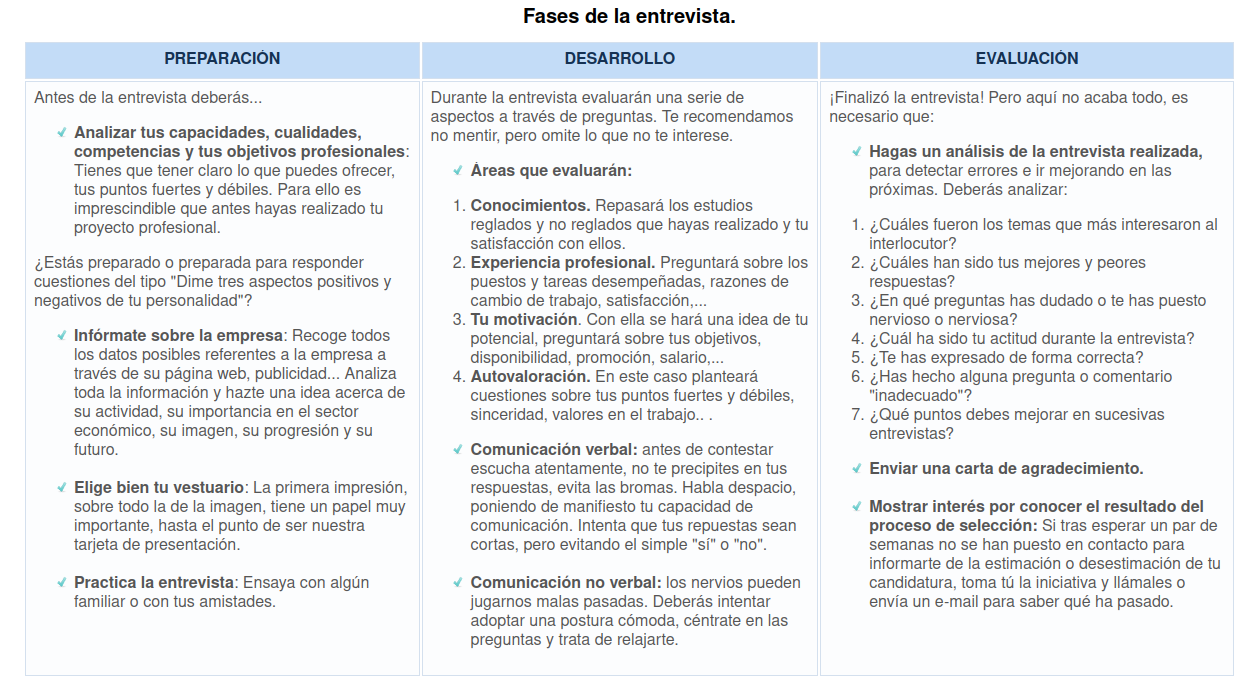
\includegraphics[scale=0.45]{fases-entrevista.png}
    \caption{Fases de una entrevista de selección}
\end{figure}

Ahora que ya tienes una idea sobre que es una entrevista de selección y cuales son sus fases, te recomendaríamos que practicaras con algún familiar o amigo estás entrevistas para que te vayas acostumbrando y afrontes una real con mayor tranquilidad.

\subsubsection{Pruebas de Selección}
Además de la entrevista de selección, la empresas pueden utilizar \textbf{pruebas de selección} en sus procesos de selección. Éstas pueden ser posteriores o anteriores a la entrevista de selección.

La finalidad de estas pruebas es medir una serie de características personales, conductuales o profesionales de los candidatos para determinar la adecuación al puesto de trabajo. Con ellas se obtiene información de las competencias, capacidades, inteligencia, habilidades, conductas, rasgos de personalidad, etc...

Las pruebas pueden ser de diferente índole, como escritas, test de desarrollo práctico-profesional, técnicas de simulación de situaciones, etc..

Los tipos mas comunes que nos podemos encontrar son los siguientes:

\begin{itemize}
    \item \textbf{Test de Proyectos}: buscan predecir el comportamiento futuro de una persona. Tratan de revelar los aspectos más escondidos de la personalidad de un candidato, como mal control de sus emociones, falta de iniciativa, excesiva ambición,..
    \item \textbf{Test de Aptitudes}: valoran los requisitos específicos del candidato/a para un determinado puesto de trabajo. Este test trata de medir diferentes funciones como el tiempo de reacción, la coordinación...
    \item \textbf{Test de Inteligencia}: valoran el nivel intelectual así como diferentes factores relacionados con la inteligencia. Es usual someter al candidato/a a una batería de preguntas contra el tiempo, donde se le pide hacer secuencias lógicas o escribir una serie de palabras por minuto.
    \item \textbf{Test de Personalidad}: miden características personales del candidato como autocontrol, emocionalidad, iniciativa,... Se le pregunta que responda a una serie de preguntas, bien diciendo si o no, o dando una respuesta libre espontánea.
    \item \textbf{Pruebas Profesionales}: sirven para estudiar las competencias del candidato relacionadas con el puesto de trabajo.
    \item \textbf{Pruebas Físicas y Médicas}: se utilizan para determinar el estado físico y de salud del candidato.
    \item \textbf{Dinámicas de Grupo}: consiste en exponer a los candidatos/as ante diferentes situaciones para que interactúen entre ellos, evaluando la capacidad de comunicación, de liderazgo, el rol que asume una persona dentro de grupo, etc..
\end{itemize}

Por último, cabe destacar, que en el sector de las nuevas tecnológicas, especialmente para los \textbf{puestos} relacionados con el \textbf{desarrollo de software}, casi siempre nos encontraremos con \textbf{pruebas técnicas}, donde nos propondrán la realización de un ejercicio de software para ver como lo resolvemos y si tenemos los conocimientos necesarios para cubrir el puesto.

\subsection{Trabajar en Europa}
La \textbf{libre circulación de trabajadores} es uno de los principios fundamentales de la Unión Europea. Esto significa que cualquier ciudadano de la UE puede trabajar en cualquiera de los estados miembros en igualdad de condiciones, con los mismos derechos y obligaciones independientemente de cuál sea su país de origen.

Si tienes interés en trabajar en Europa al acabar el Ciclo Formativo, es importante que conozcas los recursos de internet que la Unión Europea pone a disposición de sus ciudadanos para facilitar esta tarea.

\begin{itemize}
    \item \textbf{EURES: Portal Europeo de la Movilidad Profesional}: este portal tiene como objetivo servir de enlace entre los distintos servicios públicos de empleo de la UE. A través de su página web puedes acceder a una base de datos común con ofertas de empleo y convocatorias en toda la UE. Puedes visitar la plataforma EURES en este enlace:
    \begin{itemize}
        \item \href{https://eures.ec.europa.eu/index_es}{Plataforma EURES}.
    \end{itemize}

    Desde la web también se puede acceder a aspectos prácticos sobre el trabajo y la vida en los diferentes países, como características del mercado laboral, legislación, etc...

    \vspace{5ex}

    \item \textbf{Tu Europa}: esta página de la Comisión Europea ofrece información útil sobre cualquier país de la Unión Europa: fiscalidad,  derechos, seguridad social, trámites, reconocimiento de titulaciones...
    datos común con ofertas de empleo y convocatorias en toda la UE. Puedes visitar la plataforma EURES en este enlace:
    \begin{itemize}
        \item \href{https://ec.europa.eu/youreurope/citizens/index_es.htm}{Tu Europa}.
    \end{itemize}

    \item \textbf{Portal Europeo de la Juventud}: el objetivo de este portal es promover el trabajo, la ciudadanía activa y la solidaridad entre los jóvenes de la UE. Podrás encontrar información relativa al trabajo, voluntariado, intercambio,... entre los jóvenes de la UE.
        \begin{itemize}
        \item \href{https://youth.europa.eu/go-abroad/working_es}{Portal Europeo de la Juventud}.
    \end{itemize}

    Si pinchas en el menú de la izquierda, \textbf{Trabajar}, accederás a un directorio con páginas web relacionadas con el trabajo.
\end{itemize}

Por último, hay que recordar que deberás utilizar el \textbf{modelo de currículum europeo} cuando encuentres una oferta a la que quieras presentarte. Este currículum podrás encontrarlo en la página de \href{https://europa.eu/europass/es/create-europass-cv}{Europass}, plataforma que contiene un dossier de documentos cuyo objetivo es facilitar la movilidad de trabajadores en los países miembros de la UE.

\subsection{Trabajar en la Administración Pública}
Ya sabes que una de las formas de trabajar es en la Administración Pública. Si es el camino que has decido tomar, es conveniente tener alguna información y conocer algunos recursos básicos para facilitar la tarea.

Aproximadamente un 15\% de la población activa trabaja para diferentes administraciones publicas españolas: Comunidades Autónomas, Ayuntamientos, Estado Central,.. Trabajar en la administración tiene sus ventajas, pero también sus inconvenientes, como podemos ver en la siguiente figura.

\begin{figure}[ht]
    \centering
    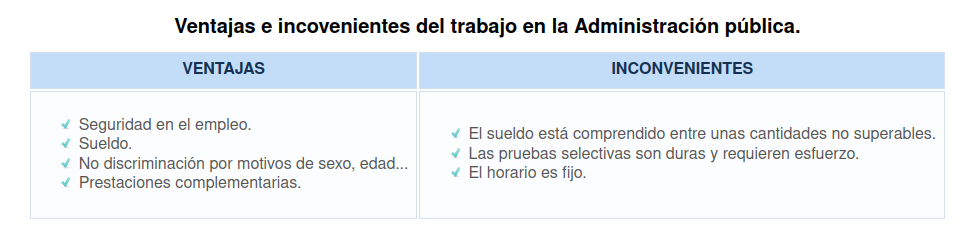
\includegraphics[scale=0.60]{ventajas-funcionario.png}
    \caption{Ventajas e Inconvenientes de trabajar con la Administración Pública}
\end{figure}

Aprobar una oposición no es fácil. No basta con estudiar y practicas sino que hay que tener una gran fuerza de voluntad para no desanimarse. Es imprescindible que sepas que puestos ofrece el ámbito público, cual es el temario, que tipo de pruebas se llevarán a cabo, o cuales son los \textbf{méritos baremables} en el caso de que sea un concurso de oposición público, entre otras cosas. Para ello deberás deberás realizar una primera labor de búsqueda de información, para ello, vamos a refrescar las salidas profesionales del ámbito público que ya hemos visto anteriormente en esta unidad.

Como recordarás, en el ámbito público tienes acceso a los puestos de \textbf{Técnicos Auxiliares Informáticos} de la Administración del Estado o las Autonómicas. Es aconsejable que busques diferentes oposiciones que te interesen y analices cual es el temario, los tipos de pruebas, que méritos son baremables y la creación de bolsas de trabajo.

Para informarte de que oposiciones se convocan y otra información referente a este tema puede consultar alguno de los siguientes enlaces:

\begin{itemize}
    \item \href{https://administracion.gob.es/pag_Home/empleoPublico/boletin.html}{Boletín Semanal de Empleo Público}
    \item \href{https://www.empleopublico.net/}{Empleopublico.net}
    \item \href{https://www.oposiciones.net/}{Oposiones.net}
    \item \href{https://www.juntadeandalucia.es/institutodeadministracionpublica/institutodeadministracionpublica/publico/home.filter?idsitio=15}{Instituto Andaluz de Administraciones Públicas}
\end{itemize}

Por último, recordarte que en el \textbf{Anexo A.3} encontrarás información mas detallada sobre los diferentes tipos de relaciones laborales que se pueden entablar con la Administración Pública.

\section{Seguir Formándose: Importancia de la Formación Permanente}
La motivación y la formación son cuestiones clave que se deben abordar desde una perspectiva contextualizada en la sociedad actual. El mercado laboral cambiante y las nuevas necesidades hacen que \textbf{clave} una permanente \textbf{actualización de los conocimientos} y formación, ya que de otra forma estos quedarán obsoletos de forma rápida.

Tantos los cursos pequeños ligados a las TIC, hasta los cursos específicos relacionados con oficios o la profesión a ejercer nos sitúan mejor posicionados para afrontar las oportunidades que se nos presenten. Por ello, vamos a analizar las diferentes opciones formativas que podemos encontrarnos tras acabar un Ciclo Formativo, sin olvidar que hay que \textbf{estar continuamente formándose} para actualizar los conocimientos y ser competitivo.

\subsection{Estudios Universitarios}
Aunque la finalidad de la Formación Profesional Específica es formar profesionales preparados para su incorporación al mercado laboral, los titulados en Ciclos de Formación de Grado Superior pueden cursar otros estudios superiores como son los universitarios. En este aspecto, el \textbf{título de Técnico Superior} ofrece acceso directo a la universidad. En función del título que se haya cursado, se podrá acceder a unos u otros estudios universitarios.

En concreto, los Ciclos Formativos de \textbf{DAM},\textbf{DAW} y \textbf{ASIR}, permiten el \textbf{acceso} de diferentes \textbf{titulaciones de informática}, como el Grado en Ingeniería Informática, Grado en Ingeniería Informática del Software, Grado en Ingeniería Informática de Servicios y Aplicaciones, etc...

En lo referente al \textbf{acceso}, el \href{https://www.boe.es/diario\_boe/txt.php?id=BOE-A-2014-6008}{Real Decreto 412/2014} establece toda la normativa básica de los procedimientos de admisión a las enseñanzas oficiales de Grado y los procedimientos de admisión en las universidades públicas españolas.

También hay que recordar que al acceder a estudios universitarios desde un Ciclo Formativo Superior \textbf{sistema de convalidaciones}, que establece:

\begin{enumerate}
    \item Las convalidaciones entre quienes posean el título de Técnico Superior, y cursen enseñanzas universitarias de grado relacionadas con dicho título, serán de al menos, 30 créditos ECTS.
    \item Siempre que las enseñanzas universitarias de grado incluyan prácticas externas en empresas de similar naturaleza a las realizadas en los ciclos formativos, se podrán convalidar, además, los créditos asignados al módulo profesional de Formación en Centros de Trabajo del título de Técnico Superior relacionado con dichas enseñanzas universitarias.
    \item Se podrán también convalidar otros créditos teniendo en cuenta la adecuación entre las competencias y conocimientos asociados a materias conducentes a la obtención de títulos de grado, o equivalente, con créditos obtenidos en los módulos profesionales superados del correspondiente título de Técnico Superior.
\end{enumerate}

\subsection{Estudiar otro Ciclo Formativo}
Otra posibilidad es estudiar ciclos formativos relativos a la familia que ya hemos estudiado, ya que nos permiten adquirir otra especialidad con relativa facilidad, al tratarse de estudios con contenidos similares, pudiendo convalidar las asignaturas comunes entres los diferentes Ciclos Formativos.

En nuestro caso, las titulaciones que entran dentro de este grupo son las que hemos visto durante este tema, \textbf{Técnico Superior en Desarrollo de Aplicaciones Multiplataforma}, \textbf{Técnico Superior en Desarrollo de Aplicaciones Web} y \textbf{Técnico Superior en Administración de Sistemas Informáticos en Red}.

\subsection{Formación Profesional para el Empleo}
La \textbf{Formación para el empleo} es el conjunto de instrumentos y acciones que tienen por objeto impulsar y extender entre las empresas y los trabajadores ocupados y desempleados una formación que responda a sus necesidad. Esta formación se integra dentro del Sistema de Formación Profesional, al igual que la Formación Inicial, constituida por los ciclos formativos de grado medio y superior del Sistema Educativo.

La Formación Profesional para el Empleo se articula en cursos o acciones formativas integradas en Familias Profesionales y esta dirigida a \textbf{trabajadores}, ya estén ocupados o desempleados, de deseen cualificarse, re-cualificarse o especializarse para mejorar sus oportunidades de acceso o permanencia en el mercado laboral.

Existe una extensa oferta formativa, tanto en modalidad presencial, como a distancia, mixta y teleformación. Los cursos suelen tener una duración variables, si bien los mas extensos no superan el año de duración. Ademas, estos cursos están financiados/subvencionados por las Administraciones Públicas, siendo la mayoría de ellos gratuitos.

Estos cursos \textbf{son ofertados} por las \textbf{Administraciones Públicas}, \textbf{Sindicatos}, \textbf{Organizaciones Empresariales} y \textbf{Centros} de formación \textbf{privados}. En el caso de asociaciones empresariales y sindicatos no es necesario estar afiliado, ya que estos cursos se financian en parte con las cuotas de todos los trabajadores.

Los \textbf{cursos de especialización} son otra opción, concretamente en la familia de informática podemos encontrar los siguientes:

\begin{itemize}
    \item \href{https://www.todofp.es/que-estudiar/loe/informatica-comunicaciones/ce-inteligencia-artificial-bigdata.html}{Curso de Especialización en Inteligencia Artificial y Big Data}
    \item \href{https://www.todofp.es/que-estudiar/loe/informatica-comunicaciones/ce-desarrollo-videojuegos-realidad-virtual.html}{Curso de Especialización en Desarrollo de Videojuegos y Realidad Virtual}
    \item \href{https://www.todofp.es/que-estudiar/loe/informatica-comunicaciones/ciberseguridad-entornos-tecnologias-informacion.html}{Curso de Especialización en Ciberseguridad en Entornos de las Tecnologías de la Información}
\end{itemize}

Además de los cursos de formación para el empleo, las \textbf{entidades privadas ofertan cursos} que pueden ayudarte a especializarte y profundizar en las áreas que más te interesen. Para saber que centros imparten un curso determinado, solo tienes que buscar el curso en cualquier buscador de internet y te aparecerán muchos resultados.

\subsection{Estudiar en Europa}
Cada vez son más los alumnos que deciden estudiar o realizar la prácticas de Formación en Centros de Trabajo en otro país europeo. Esto te permitirá adquirir nuevas competencias lingüísticas, así como conocer otra cultura y hacer amigos de diferentes países. Además, es positivo para tu currículum.

A continuación listamos un conjunto de recursos web que te serán de gran utilidad si te has decidido por esta opción:

\begin{itemize}
    \item \textbf{\href{https://spain.representation.ec.europa.eu/index_es}{PLOTEUS}} (Portal on Learning Opportunities Throughout the European Space): este portal contiene información sobre las oportunidades de aprendizaje en el espacio europeo. Tiene como objetivo ayudar a estudiantes, trabajadores, padres, orientadores y profesores a encontrar información sobre las opciones de aprendizaje a lo largo de la vida en Europa. Se estructura en la siguientes secciones:
    \begin{itemize}
        \item \textbf{Oportunidades de Aprendizaje y Posibilidades de Formación}: contiene múltiples enlaces a páginas web de universidades e instituciones de enseñanza superior, bases de datos de centros escolares y formación profesional, así como cursos de enseñanza para adultos.
        \item \textbf{Sistemas de Educación y Formación}: contiene información sobre los distintos sistemas de enseñanza y formación de los países europeos.
        \item \textbf{Programas de Intercambio y Becas}: contiene información sobre todas las becas y programas de intercambio que podemos solicitar, entre los que se encuentran los programas ERASMUS, Leonardo da Vinci, Sócrates y Tempus entre otros.
        \item \textbf{Vivir en el Extranjero}: sección con información sobre todo lo que debes saber cuando te trasladas a otro país de la UE, como coste de vida, gastos de educación, alojamiento, marco legal, y otra información general sobre los países europeos.
    \end{itemize}
    \item \textbf{\href{https://www.estudiareneuropa.eu/}{Estudiar en Europa}}: en esta página se ofrece información sobre cursos y programas, estudios superiores, así como toda la información que necesitas conocer para iniciar tu aventura europea.
    \item \textbf{\href{https://youth.europa.eu/home_es}{Portal Europeo de Juventur}}: en esta plataforma se recogen todas las oportunidades y posibilidades para estudiar en Europa, especialmente enfocada a la gente joven.
\end{itemize}

Entre todas estas opciones, cabe destacar el \textbf{Programa Erasmus}, uno de los más conocidos y que permite la realización de una parte de las prácticas de FTC en otro país europeo. Para más información, consulta con tu centro de estudios.

% Apéndice
\appendix

% Change appendix display options
\titleformat{\chapter}{\bfseries\Huge}{\thechapter.}{1ex}{}

\chapter{Anexo Tema 1}

\section{Proyecto Profesional}
En este anexo vamos a recopilar toda la información sobre el proyecto profesional, incluyendo su estructura, diferentes documentos, etc...

\subsection{Balance Personal}
Primero debes evaluar cuales pueden ser tus aportaciones al mercado laboral, siguiendo estos pasos:

\begin{itemize}
    \item \textbf{Indica tus conocimientos y habilidades}
    \item \textbf{Explica tus experiencias profesionales}: aunque no se tenga experiencia profesional, seguro que se han realizado actividades en las que se han demostrado capacidades útiles de cara al trabajo, como actividades de voluntariado, ayuda en el negocio familiar, etc.. En la siguiente figura se muestra un esquema que puede resultar de ayuda:

    \begin{figure}[ht]
        \centering
        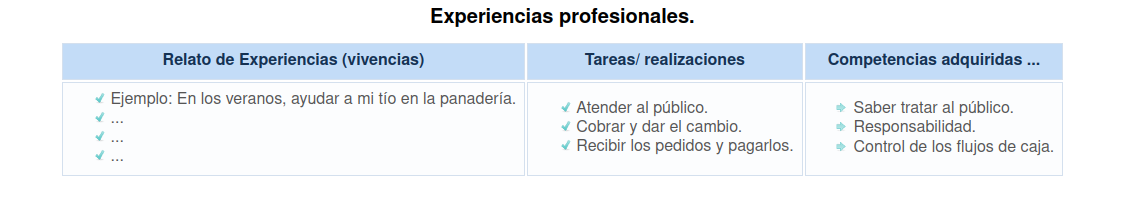
\includegraphics[scale=0.50]{experiencia-prof.png}
        \caption{Proyecto Profesional: Experiencia Profesional}
    \end{figure}

    \item \textbf{Aspecto positivos y negativos de tu personalidad}: indica, en un esquema como el de la siguientes figura, 5 aspectos positivos y negativos de tu personalidad. También puedes pedirle a alguien que te conozca bien que los escriba, para que sean lo mas subjetivos posible.

    \begin{figure}[ht]
        \centering
        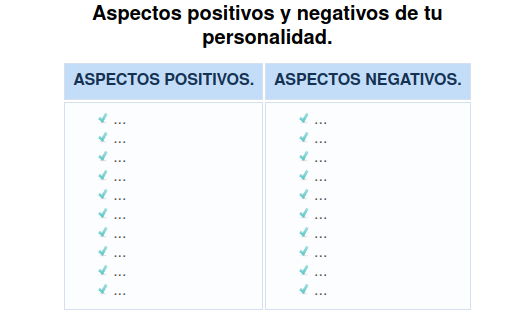
\includegraphics[scale=0.50]{aspectos-pos.png}
        \caption{Proyecto Profesional: Aspectos Personalidad}
    \end{figure}

    \item \textbf{Valores de trabajo que posees}: crea una tabla como la siguiente y rellénala con los valores que posees y que pueden aportarte valor como empleado.

    \begin{figure}[ht]
        \centering
        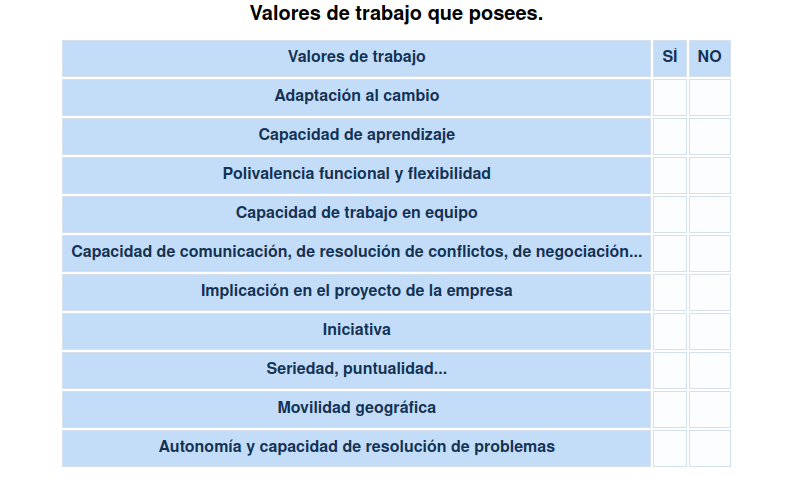
\includegraphics[scale=0.50]{valores-trabajo.png}
        \caption{Proyecto Profesional: Valores de Trabajo}
    \end{figure}
\end{itemize}

\subsection{Analisis de Mercado}
Realiza una búsqueda de ofertas de empleo y rellena un cuestionario como el que se muestra a continuación:

\begin{figure}[ht]
    \centering
    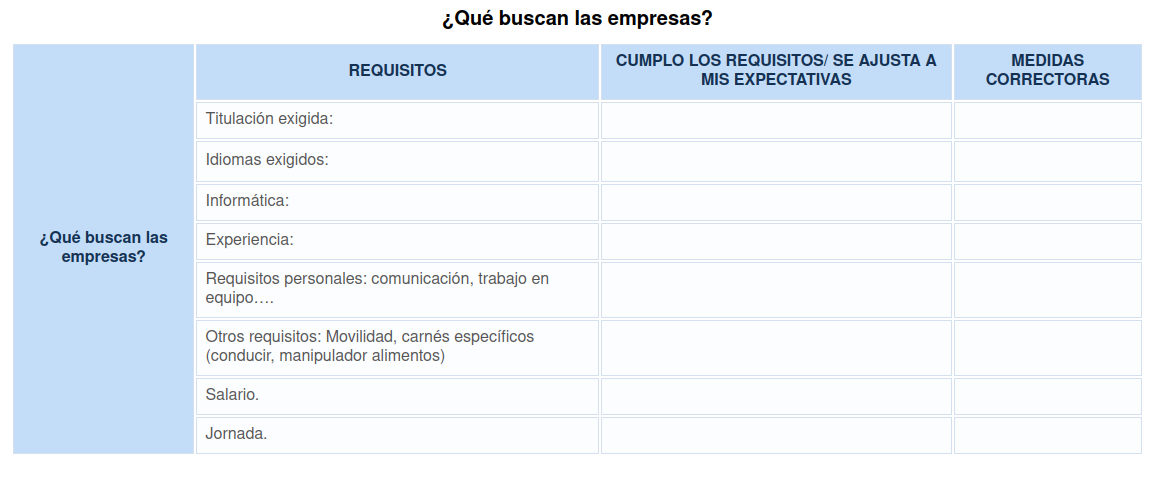
\includegraphics[scale=0.50]{estudio-mercado.png}
    \caption{Proyecto Profesional: Estudio de Mercado}
\end{figure}

\subsection{Objetivo Profesional}
El siguiente paso es definir cual es tu objetivo profesional. Para ello sigue estos pasos:

\begin{itemize}
    \item \textbf{Definir el objetivo}: define cual es tu meta, es decir, que puesto/s te gustaría ocupar.

    \item \textbf{¿Que necesito para conseguir?}: analiza y busca información sobre que \textbf{requisitos} tanto \textbf{formativos} como de \textbf{experiencia} se suelen requerir en ese puesto, elabora una lista con estos requisitos así como otros aspectos que necesites para conseguir tu objetivo.

    \item \textbf{Medidas Correctoras}: a partir de la lista anterior, elabora otra con el conjunto de \textbf{medidas} que vas a adoptar para \textbf{mejorar} aquellos aspectos en los que hayas detectado \textbf{carencias}.

    \item \textbf{Condiciones laborales}: determina las preferencias relativas a las condiciones laborales que esperas así como cuales estás dispuesto a aceptar. Elabora una tabla como la que se muestra en la siguiente figura.
    \begin{figure}[ht]
        \centering
        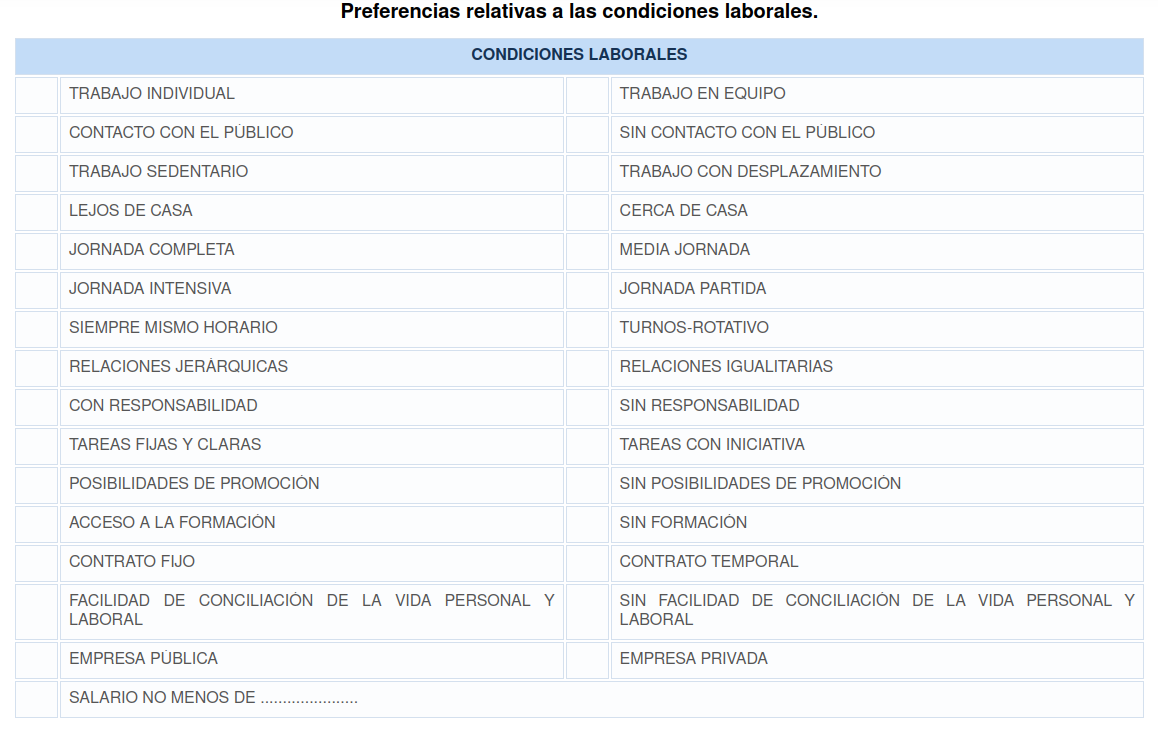
\includegraphics[scale=0.45]{condiciones-laborales.png}
        \caption{Proyecto Profesional: Condiciones Laborales}
    \end{figure}

    \item \textbf{Pasos a Seguir}: elabora una lista con los pasos que deberás seguir para la consecución del objetivo final, que es conseguir un empleo en el puesto deseado.

    \item \textbf{Alternativas}: por si falla el plan, elabora una lista con alternativas.
\end{itemize}

\section{Tipos de Currículum y Estructura}
En este anexo se profundiza más en los tipos de currículum que podemos encontrar en la estructura básica que deber tener cualquier currículum

\subsection{Tipos de Currículum}
Los tipos de currículum mas comunes son los siguientes:

\begin{itemize}
    \item \textbf{Currículum Vitae Cronológico}

    Es el más utilizado es muy buen recibido por los seleccionadores de empleo que buscan estudiar tu personalidad  a través de los mismos. Permite presentar la información de lo mas antiguo a lo más reciente y tiene la \textbf{ventaja} de \textbf{resaltar la evolución} seguida. Tiene el \textbf{inconveniente} de que las \textbf{primeras experiencias} son \textbf{menos relevantes} y las \textbf{lagunas en el tiempo} se \textbf{resaltan más}. Es interesante usar este modelo siempre que:

    \begin{itemize}
        \item Tus puestos de trabajo han evolucionado por orden cronológico y dentro de una misma línea.
        \item Has tenido pocos trabajos y con funciones idénticas o muy similares.
        \item No quieres cambiar la línea de trabajo.
    \end{itemize}

    \item \textbf{Currículum Cronológico Inverso}

    Este modelo de currículum, que gana cada día mas adeptos, consiste en presentar el currículum en orden cronológico pero con los eventos mas recientes en primera instancia. Tiene la \textbf{ventaja} que \textbf{resalta} las \textbf{experiencias más recientes}, que al final son las más importantes.

    \item \textbf{Currículum Vitae Funcional}

    En este modelo se distribuye la información por temas y proporciona un conocimiento rápido de tu experiencia y formación en un ámbito concreto. No sigue un orden cronológico, por lo que permite resaltar los puntos positivos, trabajos y funciones acordes al puesto que solicitas, más que su evolución. También permite omitir los eventuales errores de recorrido, los periodos de paro, frecuentes cambios de trabajo,... Este currículum se escribe pensando en las exigencias de un puesto determinado y dando respuesta a las necesidades de al empresa. Es importante antes de comenzar a redactarlo, tener bien claro los siguientes puntos:

    \begin{itemize}
        \item Tu objetivo ocupacional.
        \item Las experiencias, funciones y logros que se relacionen con tu objetivo profesional.
        \item Empresas en las que hayas realizado funciones requeridas para la consecución de tu objetivo.
        \item La formación académica, así como cursos y seminarios relacionados con tu objetivo.
        \item Este modelo destaca la diferencias que poseer para ocupar un puesto en particular y es \textbf{especialmente útil} cuando tu \textbf{experiencia no esta relacionada} con el puesto al que te estas presentando, cuando estas optando por un \textbf{cambio de carrera profesional}, cuando reingresas al \textbf{mercado laboral} tras un tiempo de paréntesis o cuando estás entrando al mercado laboral por primera vez.
    \end{itemize}
\end{itemize}

\subsection{Estructura del Currículum}
Cualquier currículum debe incluir, como mínimo, los siguientes puntos:

\begin{enumerate}
    \item \textbf{Datos Personales}: nombre y apellidos, lugar de nacimiento, nacionalidad (si no es española), dirección personal, teléfono de contacto y correo electrónico.

    \item \textbf{Formación Académica}: estudios reglados realizados relativos al perfil solicitado por la empresa, indicando el centro y la localidad de realización y fechas. Se deben incluir solo los estudios de más alto nivel, no siendo necesario incluir la educación secundaria. Tampoco se debe hacer referencia a las calificaciones obtenidas.

    \item \textbf{Formación Complementaria}: estudios no reglados como cursos o seminarios, indicando centro y horas lectivas, que sean relativos al puesto que se quiere ocupar.

    \item \textbf{Idiomas}: conocimientos de idiomas precisando el nivel oral y escrito. Si obtuviste algún título reconocido o tuviste alguna estancia en el extranjero indícalo.

    \item \textbf{Informática}: conocimientos de informática especificando el grado de domino de programas, aplicaciones y lenguajes de programación.

    \item \textbf{Experiencia Profesional}: relación de la diferentes experiencias profesionales realizadas. Es imprescindible dar el máximo detalle posible: nombre y actividad de la empresa, fechas, puestos y funciones desempeñadas. Esto permitirá a la persona que lea tu currículum evaluar rápidamente las competencias. En caso de no tener experiencia incluye las prácticas que hayas realizado durante tus estudios y las actividades de voluntariado.

    \item \textbf{Datos de Interés}: datos no incluidos en los apartados anteriores, pero solo aquellos que aporten información relevante sobre tu perfil y puedan aumentar el valor de tu currículum: premios literarios, carnet de conducir, vehículo propio, disponibilidad para viajar, etc..
\end{enumerate}

\section{Tipos de Relaciones con la Administración}
Los tipos de relaciones que se pueden establecer con las Administración Pública son los siguientes:

\begin{itemize}
    \item \textbf{Funcionario de Carrera}: personal de plantilla de la Administración Pública que presta sus servicios de forma permanente. Se trata de relaciones reguladas por el Derecho Administrativo.

    \item \textbf{Funcionario Interino}: son personal funcionario de empleo interino quienes, por razones expresamente justificadas de necesidad y urgencia, son nombrados como tales para el desempeño de las labores de los funcionarios de carrera, cuando se de alguna de las siguientes circunstancias:

    \begin{itemize}
        \item La existencia de plazas vacantes cuando no sea posible su cobertura por funcionarios de carrera.
        \item La sustitución transitoria de las personas titulares de la plaza.
        \item La ejecución de programas de carácter temporal.
        \item El exceso o acumulación de tareas por plazo máximo de 6 meses dentro de un período de 12 meses.
    \end{itemize}

    \item \textbf{Personal Laboral}: son aquellos trabajadores asalariados contratados por la Administración Pública, cuya relación es regulada por el Derecho Administrativo y los convenios colectivos. Sus contratos pueden ser indefinidos o de duración limitada. Las categorías profesionales de estos trabajadores son las que fijan los convenios y se fijan en función de la titulación exigida para la convocatoria.

    \item \textbf{Personal Eventual}: son quienes, en virtud de nombramiento y con carácter no permanente, solo realizan funciones expresamente calificadas como de confianza o asesoramiento especial, retribuyéndoseles con cargo a los presupuestos consignados a este fin.
\end{itemize}

\section{Formas de Acceso a Empleo Público}
Las formas de acceso al empleo pública son las siguientes:

\begin{itemize}
    \item \textbf{Contratación temporal bajo presupuesto de programas específicos}: las entidades públicas pueden solicitar programas que incluyan la contratación de personal. Hay que tener en cuenta que estos contratos duran exclusivamente lo que dura el programa, y no hay obligatoriedad de vinculación posterior con la entidad.

    \item \textbf{Bolsas de trabajo por concurso de méritos}: las Administraciones pueden hacer pública una necesidad de personal, haciendo una baremación de méritos (títulos, cursos realizados, experiencia laboral).

    \item \textbf{Oposiciones}: una oposición es un procedimiento selectivo consistente en una o más pruebas elaboradas sobre un temario oficial, en que los aspirantes a un puesto de trabajo muestran sus respectivas competencias, juzgadas por un tribunal. Estas pruebas suelen ser duras, debes de tener claro que quieres preparártelas antes de hacer la inversión de tiempo y esfuerzo. También debes considerar que muchas oposiciones comparten parte del temario, así que con un poco de esfuerzo extra puedes presentarte a distintas plazas. Lo mejor es considerar esta opción como un objetivo a conseguir a medio y largo plazo. Estos puestos de trabajo son ofrecidos a través de convocatorias por las Administraciones Públicas, de ahí que estas ofertas de empleo se denominen Ofertas de Empleo Público (OPE), publicadas en los Boletines Oficiales del Estado, Autonomías y Provincias.

    En muchas de ellas, las convocatorias establecen la posibilidad de crear listas de interinidades/bolsas de trabajo con aquellos aspirantes que no hayan obtenido plaza o no hayan superado el proceso selectivo, de tal forma que cuando se precise personal para cubrir una incapacidad temporal de un titular o por existir una vacante, se llamará a las personas de esa bolsa.

    \item \textbf{Concurso-Oposición}: Al igual que en la oposición consiste en pruebas selectivas elaboradas sobre un temario oficial, no obstante en este caso la calificación final vendrá determinada no sólo por la nota del examen o prueba de conocimientos, sino también por los méritos.
\end{itemize}

Los méritos vendrán determinados por experiencia en puestos de la misma categoría a la que se opta, titulaciones oficiales y los denominados ``\textbf{cursos baremables}''. Fíjate bien en ellos, porque estos cursos te pueden dar la llave al empleo, ya que otorgan puntos para la oposición. Son cursos aceptados por las diversas Administraciones en sus convocatorias de Empleo Público y en las diversas bolsas de trabajo. Son impartidos por sindicatos, organizaciones empresariales, Comunidades Autónomas... Lee bien la convocatoria e infórmate en el organismo que las convoca qué cursos son baremables y dónde los puedes realizar. Por último al igual que en las oposiciones es habitual que en esta forma de acceso la convocatoria establezca la creación de listas de interinidades/ bolsas de trabajo o sustituciones.

% Glossary
\glsaddall
\printglossaries

% Bibliography
\newpage
\addcontentsline{toc}{chapter}{Bibliografía}
\bibliography{citas}
\bibliographystyle{unsrt}

\end{document}